\documentclass[12pt,a4paper]{article}
\usepackage[T1]{fontenc}
\usepackage{polski}
\usepackage[utf8]{inputenc}
%\usepackage[cp1250]{inputenc}
\usepackage[french,polish]{babel}
\usepackage{graphicx}
\usepackage{ulem}
\usepackage{amsmath}
\usepackage{epstopdf}
\usepackage{gensymb}
\usepackage{polski}
\usepackage{fontspec}
\usepackage{xunicode}
\usepackage{xltxtra}
\setmainfont[Mapping=tex-text]{Georgia}
\usepackage[acronym, toc]{glossaries}
\usepackage{lmodern}
\usepackage[rgb]{xcolor}
\usepackage[author={Michał Małaj}]{pdfcomment}




\title{SKRYPT SZKOLENIOWY SZKOLENIE "FOTOWOLTAIKA W BUDOWNICTWIE"}
\author{w ramach projektu: \textit{"Praca szansą na osobisty rozwój"} } 
\date{\today}
\begin{document}
\maketitle
\tableofcontents

\section{Moduł 1 Panele fotowoltaiczne w kontekście technologii odnawialnych. }

\subsection{Co to jest układ fotowoltaiczny? }
Skrót PV (z j. ang. photovoltaic) oznacza fotowoltaiczny, czyli zdolność 
materiału do wytwarzania napięcia, zwykle dzięki fotoemisji, w warunkach 
ekspozycji na energię promieniowania, szczególnie światła. 

Proces konwersji światła (fotonów) bezpośrednio na elektryczność 
(napięcie) jest nazywany fotowoltaiką (PV = photovoltaics). Kiedy 
materiały fotowoltaiczne absorbują światło słoneczne, wybija ono 
elektrony, uwalniając je z atomów, umożliwiając im płynięcie przez 
materiał i wytwarzanie elektryczności. 

Materiały fotowoltaiczne używane są do budowy ogniw słonecznych, które 
na ogół są zgrupowane w moduły fotowoltaiczne (znane także jako panele 
słoneczne). Moduły mogą być wzajemnie pogrupowane i połączone tworząc 
generatory fotowoltaiczne (pola modułów). 

Na układ PV składa się kilka elementów składowych: panele słoneczne, 
system montażu, inwerter (falownik), licznik energii, okablowanie, układ 
sterowania, tablica rozdzielcza. 

\subsection{Korzyści z układów fotowoltaicznych }

Z instalacją PV wiąże się z kilka rodzajów korzyści. Dwa główne to 
ekonomiczne i środowiskowe. Za korzyść ekonomiczną faktycznie uważa się 
inwestycją, która co prawda wymaga poniesienia pewnego kosztu 
początkowego związanego z uruchomieniem systemu PV, ale potem system ten 
będzie potrzebował bardzo niewiele zabiegów konserwacyjnych, a będzie w 
sposób ciągły generował elektryczność, którą można odsprzedawać klientom 
sieciowym. \textbf{Poniżej podano kilka przykładów takich korzyści: }

\subsubsection{Ekonomiczne}

\underline{Zredukowanie wysokości rachunków za elektryczność}: 
światło słoneczne jest za darmo, więc kiedy poniesiemy początkowe koszty 
instalacji, to koszty elektryczności zostaną znacznie zredukowane. 
Typowy domowy system PV może zaspokoić zapotrzebowanie na około 40\% 
energii, jaką zużywa się rocznie w gospodarstwie domowym. 

\underline{Sprzedaż elektryczności dystrybutorowi energii elektrycznej
}: jeśli układ produkuje więcej energii elektrycznej niż potrzeba i 
może zostać zużyte, to energię tę może użyć ktoś inny - a dzięki 
systemowi PV uda zarobić się trochę pieniędzy. 

\underline{Zmagazynowanie elektryczności na okres pochmurnych dni}: 
kiedy obiekt nie jest podłączony do sieci elektrycznej, układ może 
zmagazynować nadmiar energii w akumulatorach i użyć jej wtedy gdy będzie 
jej potrzebował. 

\subsubsection{Środowiskowe}

\underline{Redukcja emisji związków węgla}: elektryczność słoneczna 
jest zieloną, odnawialną energią, przy jej wykorzystaniu nie jest 
wydzielany szkodliwy dwutlenek węgla ani inne zanieczyszczenia. W 
przypadku typowego systemu \textbf{PV można uniknąć emisji około 1200 
kg dwutlenku węgla rocznie} - co stanowi około 30 ton w trakcie 
eksploatacji systemu. 

\underline{Ochrona fauny i flory}: kopalnie węglowe wymagają dużych 
ilości wody, aby usunąć różne domieszki z węgla. W elektrowniach 
węglowych zużywa się duże ilości wody do produkcji pary wodnej oraz 
wykorzystuje się ją w układach chłodzenia. Kiedy elektrownie węglowe 
czerpią wodę z jeziora lub rzeki, to ma to wpływ na ryby i inne życie 
wodne, jak również na zwierzęta i ludzi, którzy od tych zasobów wodnych 
zależą. W tym samym czasie, w wodzie używanej przez instalacje kotłowe i 
systemy chłodzenia elektrowni gromadzą się zanieczyszczenia. Jeśli woda 
używana przez elektrownię zostanie odprowadzona do jeziora lub rzeki, 
zanieczyszczenia w wodzie mogą zaszkodzić zwierzętom i roślinom. W 
systemach PV nie zachodzą takie procesy. 

\underline{Brak odpadów}: po spaleniu węgla pozostają odpady stałe i popiół, który 
składa się głównie z tlenków metali i zasad. Średnia zawartość frakcji 
popiołu w węglu to około 10\%. Odpady stałe powstają także w kopalniach 
węglowych, kiedy oczyszcza się węgiel oraz w elektrowniach, gdy 
zanieczyszczenia powietrza są usuwane z gazów kominowych. Większość tych 
odpadów jest składowana na składowiskach odpadów i w nieczynnych 
kopalniach, chociaż obecnie pewną ilość przetwarza się na użyteczne 
produkty, takie jak cement i materiały budowlane. Tak samo jest w 
przypadku elektrowni zasilanych paliwem jądrowym, gdzie powstają odpady 
radioaktywne. Takie odpady są radioaktywne przez wiele tysięcy lat i 
muszą być przechowywane w specjalnych miejscach albo pod ziemią, albo w 
betonowych kryptach zanurzonych w wodzie i otoczonych stalą. W przypadku 
systemów PV nie ma emisji spalin czy powstawania popiołu. 

\subsection{Wady systemów PV}
Poniżej są przedstawione wady systemów PV: 

\begin{itemize}
\item Pewne toksyczne związki chemiczne, takie jak kadm czy arszenik są 
używane w procesie produkcji systemów PV. Jednak te czynniki 
środowiskowe są niewielkie i mogą być łatwo kontrolowane dzięki 
recyklingowi i odpowiedniej utylizacji. 
\item Energia słoneczna jest nieco droższa w produkcji niż energia ze 
Ľródeł konwencjonalnych, w części w związku z kosztami wytworzenia 
urządzeń PV, a w części w związku ze sprawnością konwersji urządzeń tych 
urządzeń. W miarę jak sprawność konwersji zacznie wzrastać, to koszty 
wytwarzania tych urządzeń zaczną spadać i fotowoltaika stanie się coraz 
bardziej konkurencyjna pod względem kosztów w porównaniu z paliwami 
konwencjonalnymi. 
\item Energia słoneczna jest zmiennym Ľródłem energii. W tym przypadku 
produkcja energii zależy od słońca. Może się zdarzyć, że urządzenia 
słoneczne mogą nie wytwarzać energii przez pewien okres czasu, co może 
prowadzić do niedoborów w sytuacjach, gdy duża część energii jest 
właśnie czerpana ze słońca. 
\end{itemize}

\subsection{Typy systemów PV }

Systemy fotowoltaiczne są na ogół sklasyfikowane pod względem ich 
wymogów funkcjonalnych i operacyjnych, konfiguracji podzespołów, i od 
tego jak są połączone z innymi Ľródłami energii i odbiornikami 
(urządzeniami elektrycznymi). Istnieją dwie główne kategorie: układy 
podłączone do sieci energetycznej (on-grid) i układy autonomiczne (off-grid). 

\subsubsection{PV podłączone do sieci energetycznej (on grid) }

Układy PV podłączone do sieci energetycznej są zaprojektowane w taki 
sposób, aby działać równolegle i w połączeniu z siecią energetyczną. 
Głównym elementem takiego systemu jest \textit{\textbf{inwerter (falownik)}}. Inwerter 
przemienia moc stałą produkowaną przez panele PV na moc zmienną zgodną z 
wymaganiami napięcia i mocy sieci energetycznej. Inwerter automatycznie 
zatrzymuje dostarczanie energii do sieci energetycznej, gdy sieć nie 
jest zasilana. Poniżej przedstawiono typowy układ PV zintegrowany z 
siecią energetyczną 

\begin{figure}[h]
\centering
 	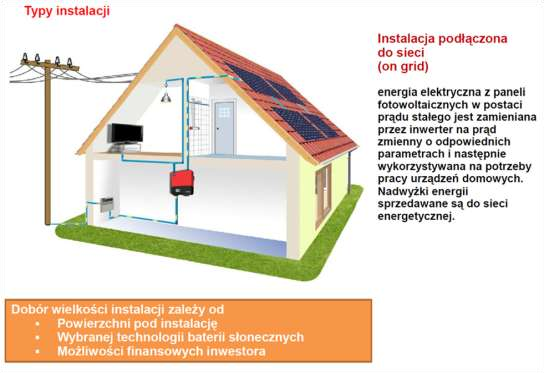
\includegraphics[natwidth=14.41cm,natheight=9.89cm]{media/image3.png}
\end{figure}

\subsubsection{Układy autonomiczne (off-grid)} 
Układy autonomiczne są zaprojektowane tak, aby działać niezależnie od 
sieci energetycznej, i są na ogół zaprojektowane tak i mają rozmiary 
odpowiednie, aby zasilać urządzenie stało- i zmiennoprądowe. Układy autonomiczne mogą być zasilane tylko przez 
generator PV albo mogą używać generatora zasilanego wiatrem lub 
zasilania sieciowego jako Ľródła zapasowego zasilania, gdzie wyjście 
stałoprądowe (DC) modułu lub generatora PV jest bezpośrednio podłączone 
do obciążenia. 

Ponieważ w takich układach nie ma urządzeń do gromadzenia energii, 
obciążenie funkcjonuje tylko w godzinach, gdy jest światło słoneczne, 
czyniąc te konstrukcje odpowiednimi dla powszechnych zastosowań jak 
wentylatory, pompy wodne i niewielkie pompy cyrkulacyjne dla solarnych 
termicznych układów ogrzewania wodą. Dopasowanie impedancji obciążenia 
elektrycznego do maksymalnej mocy wyjściowej generatora PV jest kluczową 
częścią projektowania dobrze działającego bezpośrednio sprzężonego 
systemu PV. 

Jednak w wielu autonomicznych systemach PV do magazynowania energii 
używa się akumulatorów. 

Poniżej mamy przedstawiony diagram typowego autonomicznego układu PV z 
akumulatorowym magazynowaniem energii zasilającego odbiorniki stało- i 
zmiennoprądowe. 

\begin{figure}[h]
\centering
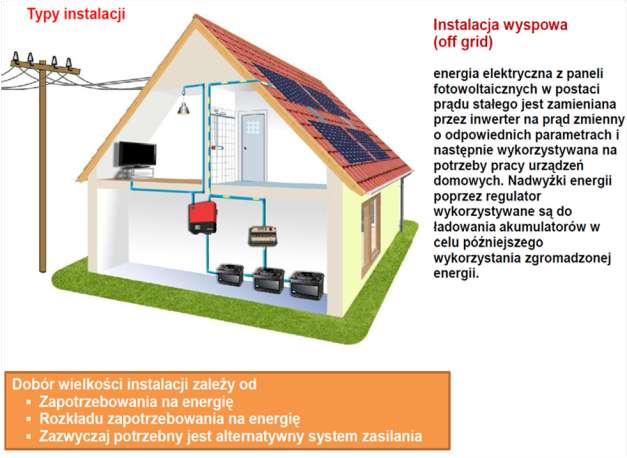
\includegraphics[natwidth=16.60cm,natheight=12.13cm]{media/image4.png}
\end{figure}

\subsection{Taryfy gwarantowane}

Taryfy gwarantowane są mechanizmem motywującym wprowadzonym przez rząd w 
celu promowania prywatnych inwestycji malej skali w zakresie technologii 
odnawialnych. Prawo obliguje dystrybutorów energii, aby płacili pewną 
kwotę za każdą produkowaną jednostkę (kWh) odnawialnej energii 
elektrycznej. Oznacza to, że początkowy nakład pieniężny wydany na 
system PV zwróci się szybciej. 

Taryfa gwarantowana ma obowiązywać przez określoną liczbę lat, co w 
przypadku fotowoltaiki ustalono na dwadzieścia pięć.

Departament Na Rzecz Zmian Energii i Klimatu \{DECC\} wydał formalne 
instrukcje (lipiec 2009) określające jak Wielka Brytania zamierza 
osiągnąć cele związane z redukcją związków węgla. Ten dokument zawiera 
ogłoszenie proponowanych taryf gwarantowanych. Ostateczne wysokości 
stawek zostały ogłoszone 1 lutego 2010 i zaczęły obowiązywać 1 kwietnia 
2010 roku.

Taryfy gwarantowane wprowadzone zostaną po 31 grudnia 2015 roku i będą 
obowiązywać przez 15 lat. 

Ma to zachęcić ludzi, aby nie czekali z inwestycją myśląc, że cena 
technologii w przyszłości spadnie: im później zainwestujesz, tym 
otrzymasz mniej zwrotu w formie taryf gwarantowanych. W ten sposób 
przedstawiono zachętę do inwestycji już teraz. Założono, że zwrot z 
inwestycji systemów PV powinien wynosić między 5 a 8 lat. \textbf{Zatwierdzone 
taryfy są zależne od mocy systemów PV i przedstawiają się następująco: 
do 3 kW - 0,75 zł/kWh; od 3 do 10 kW - 0,65 zł/kWh. }

\subsection{Zielone certyfikaty}

Zielone certyfikaty są zbywalnymi certyfikatami przyznawanymi przez 
odpowiedni organ za każdą l MWh lub 1000 kWh wyprodukowanej energii ze 
źródła odnawialnego. Są przypisane do każdej jednostki energii 
niezależnie, czy ich producent zużyje ją sam czy prześle ją do sieci 
energetycznej. Odpowiednie instytucje zajmujące się obrotem zielonymi 
certyfikatami zaczęły działać w kwietniu 2002 roku jako część 
porozumienia dystrybutorów energii elektrycznej. Porozumienie to wymaga 
od dostawców energii, aby określona część elektryczności, którą 
dostarczają swoim klientom, pochodziła ze źródeł odnawialnych. 
Rozpoczęto od 3\% w 2003 roku, podnosząc stopniowo do 10,4\% w 2010 
roku, aż do osiągnięcia 15.4\% w 2015. Koszt energii dla konsumenta ma 
być ograniczony z góry, a Zielone certyfikaty mają funkcjonować do 2027 
roku, co zostało usankcjonowane prawnie. 

Producenci spełniający niezbędne warunki otrzymują Zielone certyfikaty 
za każdą MWh wytworzonej energii. Certyfikaty te mogą zostać później 
sprzedane dostawcom, aby mogli spełnić swój obowiązek. Dostawcy mogą 
albo przedstawić wystarczającą liczbę certyfikatów, który pokrywa 
niezbędny procent ich produkcji, albo mogą zapłacić aktualną cenę wykupu 
certyfikatów za brakującą część. Wszystkie wpływy z płatności po cenie 
wykupu są zwracane dostawcom w części proporcjonalnej do liczby 
posiadanych przez nich Zielonych certyfikatów. 

Wartość Zielonych certyfikatów i taryf gwarantowanych jest corocznie 
rewidowana, a liczby używane w tych przykładach są aktualne na czerwiec 
2011. Można sprawdzić aktualne wartości na stronie OFGEM (Urząd 
Regulacji Rynków Gazu i Elektryczności) - \underline{http://www.ofgem.gov.uk}. 

\subsection{Koszty} 
Koszty instalacji systemu elektryczności solarnej mogą 
się różnić - średni system kosztuje pomiędzy 20 a 40 tysięcy złotych w 
zależności od swojego rozmiaru i typu. Cena ta zawiera cenę materiałów i 
koszty robocizny. W ogólności: 

\begin{itemize}
\item Im więcej energii elektrycznej system wytwarza, tym więcej 
kosztuje, ale można dzięki temu więcej zaoszczędzić, 
\item Dachówki fotowoltaiczne kosztują więcej niż konwencjonalne panele 
słoneczne, 
\item Zintegrowane z dachem systemy PV są na ogół droższe od systemów 
niezintegrowanych (zmodernizowanych), jednak jeśli wymagana jest większa naprawa dachu, zintegrowane płyty/panele PV mogą zrekompensować koszt pokrycia dachu.
\end{itemize}

\section{Moduł 2. Jak działa system fotowoltaiczny - zasady i budowa }
\subsection{Ogniwa, moduły i generatory PV}

Systemy fotowoltaiczne wykorzystują kilka elementów w celu konwersji 
energii światła na energię elektryczną. Najbardziej podstawowym z tych 
elementów jest \textit{ogniwo fotowoltaiczne}, które omówimy jako pierwsze. 

\subsubsection{Ogniwa}
Powszechnie używa się trzech typów ogniw: oparte na 
krzemie monokrystalicznym, polikrystalicznym (używa się też określenia 
multikrystaliczne) i krzemie amorficznym (cienkowarstwowe). Ogniwa takie są wykonane z różnych materiałów, z 
których każdy ma inne właściwości. Ogniwem o największej sprawności jest 
ogniwo monokrystaliczne, które ma czarny matowy wygląd. Ten typ ogniw ma 
sprawność konwersji energii świetlnej na elektryczność rzędu 15-18\%. 

\textbf{Ogniwa polikrystaliczne} są koloru niebieskiego z wyraźnie widocznymi 
kryształami i posiadają sprawność rzędu 10-12\%. Ogniwa z \textbf{amorficznego 
krzemu} mają sprawność 6-8\% i są na ogół koloru brązowego. Te ogniwa 
mają krótszą żywotność niż te krystaliczne, ale są tańsze z powodu ich 
cienkowarstwowej konstrukcji i redukcji surowca (mianowicie krzemu) 
potrzebnego do produkcji. Typ cienkowarstwowy ogniwa ma zaletę, że 
jest cieńszy niż typy krystaliczne i może być stosowany w szerszym 
zakresie. 
Ogniwa fotowoltaiczne funkcjonują przy \textit{niskim napięciu, typowo 0,6 V dla 
typów krystalicznych i 0,9 V dla typu z krzemu amorficznego.} Moduł jest 
zbiorem ogniw połączonych szeregowo, co sprawia, że zwiększa się 
napięcie, czyniąc moduły bardziej użytecznymi. Panel solarny jest 
modułem, który został skonstruowany z wielu ogniw. 

\begin{figure}[h]
\centering
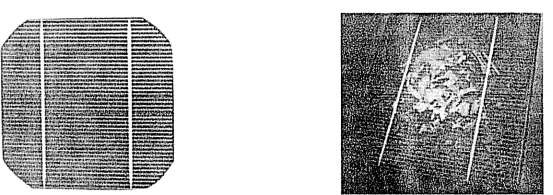
\includegraphics[natwidth=14.65cm,natheight=5.17cm]{media/image5.jpg}
\end{figure}
 ogniwo monokrystaliczne ogniwo polikrystaliczne 

\subsubsection{Moduły}
Moduł jest bardziej powszechnie znany jako panel 
solarny/słoneczny. Składa się z ogniw, które są elektrycznie połączone 
razem i zabezpieczone (przed uderzeniem gradu, wiatrem, obciążeniem 
śniegiem). Muszą również ochronić ogniwa przed wilgocią, która powoduje 
korozję metalowych kontaktów, zmniejszając ich żywotność i wydajność. 

Większość modułów jest sztywna, dzięki czemu może być przytwierdzona do 
struktury dachu budynku lub urządzeń naprowadzających na słońce. 
Połączenie elektryczne pomiędzy ogniwami są albo szeregowe, aby uzyskać 
pożądane napięcie lub/i równoległe, aby otrzymać żądane natężenie prądu 
na wyjściu. 

Moduły podlegają jakościowym wymogom produkcji takim jak standardy Unii 
Europejskiej. Poniżej przestawiono oznaczenia norm związane z wytwarzaniem modułów PV:  

PN-EN-61215:2005 - Moduły fotowoltaiczne (PV) z krzemu krystalicznego do 
zastosowań naziemnych - Kwalifikacja konstrukcji i aprobata typu. 

PN-EN-61646:2008 - Cienkowarstwowe naziemne moduły fotowoltaiczne (PV) - 
Kwalifikacja konstrukcji i zatwierdzenie typu. 

PN-EN-61730-1:2007 - Ocena bezpieczeństwa modułu fotowoltaicznego (PVJ - 
Część 1: Wymagania dotyczące konstrukcji. 

MS 005 - Wymaganie certyfikacji produktów: solarne moduły fotowoltaiczne 

\subsubsection{Generator PV, pole modułów PV} - to kolekcja elektrycznie 
połączonych modułów, które z kolei mogą być połączone szeregowo lub 
równolegle w zależności o tego, jakie napięcie lub natężenie prądu jest 
wymagane dla systemu. Wymagania systemowe są zazwyczaj podyktowane przez 
konieczne charakterystyki wejściowe dla inwertera/falownika. 

\begin{figure}[h]
\centering
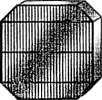
\includegraphics[natwidth=2.72cm,natheight=2.65cm]{media/image6.jpg}
\end{figure}
\begin{figure}[h]
\centering
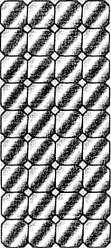
\includegraphics[natwidth=2.96cm,natheight=6.58cm]{media/image7.jpg}
\end{figure}
 \ \ \ \ \ \ \ \ \ \ \ \ ogniwo \ \ \ \ \ \ \ \ \ \ \ \ \ \ \ \ \ \ \ \ 
moduł 

\subsection{Konstrukcja modułu}

Moduły solarne obecnie są dostępne w różnych rozmiarach i kształtach. Te mogą się zmieniać od panelu solarnego do dachówek solarnych, które zastępują zwykłe dachówki. W zależności od tego, jakie moduły są zainstalowane, otrzymujemy różne parametry wyjścia. Typowy krystaliczny panel solarny 1m x 1,64m, posiada zwykle 60 ogniw dając na wyjściu przy otwartym obwodzie napięcie około 37-38 V, podczas gdy dachówka solarna złożona zwykle z 4-6 ogniw osiąga napięcie 9,6 - 21,6 V przy otwartym obwodzie. Jest całkiem jasne, że większa powierzchnia ogniw będzie produkować większą moc wyjściową naszego generatora PV. 

Ogniwa oparte na amorficznym krzemie są zbudowane inaczej. Zamiast typowego rozmieszczenia ogniw, cienka warstwa krzemu jest pocięta na paski szerokości 1cm, które posiadają napięcie przy otwartym obwodzie rzędu 0,9V. Te paski są dalej łączone razem w celu uzyskania większego napięcia wyjściowego. Typowy moduł oparty na amorficznym krzemie posiada rozmiary 3x1 stopy. Moduł takie mogłyby być krótsze, co zredukowałoby ich natężenie prądu na wyjściu albo węższe, co zredukowałoby ich napięcie na wyjściu. 

\begin{figure}[h]
\centering
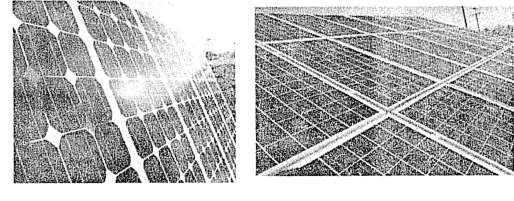
\includegraphics[natwidth=13.60cm,natheight=5.34cm]{media/image8.jpg}
\end{figure}
 

\ \ \ \ \textit{moduły z ogniwami opartymi na krzemie }\ \ \ \ 
\textit{moduły z ogniwami opartymi na krzemie }

\ \ \ \ \textit{monokrystalicznym }\ \ \ \ \textit{ }\ \ \ \ \textit{
polikrystalicznymi }

\subsection{Wpływ temperatury, oświetlenia i zacienienia na sprawność układu}

Kiedy przyjrzymy się konfiguracji modułów i generatorów PV, to należy rozważyć wiele ich parametrów. Następujące czynniki mają wpływ na sprawność generatora PV. W przypadku większości modułów podaje się ich szczytową moc wyjściową. Jest to maksymalna moc wyjściową modułów w standardowych warunkach testowych (Standard Test Conditions (STC)). 

\textbf{STC} są zdefiniowane przy poziomie natężenia promieniowania słonecznego rzędu 1000 W/m2 w temperaturze 25 stopni Celsjusza i atmosferycznej masie optycznej równej 1.5. Jest to szczytowe natężenie promieniowania i umiarkowana temperatura, co stanowi "\,idealne" warunki działania dla modułu solarnego. W rzeczywistości, występujące natężenie promieniowania jest znacznie mniejsze niż wartość szczytowa, a występująca temperatura jest zazwyczaj większa niż ta na poziomie STC. 

\underline{Na STC wpływają 4 czynniki:} 
\subsubsection{Oświetlenie}

\textbf{Oświetlenie:} (natężenie światła słonecznego), ta wielkość jest mierzona w watach na metr padające na płaską powierzchnię. Standardowy pomiar to 1000 W/m2, (jak powyżej) 

\begin{figure}[h]
\centering
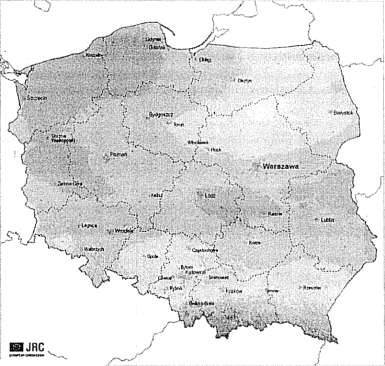
\includegraphics[natwidth=10.21cm,natheight=9.71cm]{media/image9.jpg}
\end{figure}
 

\textit{Potencjał elektryczności wytworzonej z optymalnie ustawionych 
modułów PV dla Polski (mapa pochodzi z \underline{
http://re.jrc.ec.europa.eu/pvgis/cmaps/eu\_opt/pvgis\_solar\_optimum\_PL.png
}) }

\subsubsection{Atmosferyczna masa optyczna}
\textbf{Atmosferyczna masa optyczna:} to odnosi się do "\,grubości" i przezroczystości powietrza przez, które światło słoneczne musi przejść, aby dotrzeć do modułów. Kąt padania promieni słonecznych wpływa na tę wartość. Standardową wartością jest 1,5. 
\subsubsection{Temperatura ogniwa}
\textbf{Temperatura ogniwa:} ta różni się od temperatury otaczającego powietrza. Wartość standardowych warunków testowych jest zdefiniowana jako 25 stopni Celsjusza. Sprawność systemu PV zmniejsza się wraz ze wzrostem temperatury, co z kolei ma wpływ na typ używanego systemu mocowania. 
\subsubsection{Zacienienie}
\textbf{Zacienienie:} sprawność również jest uzależniona od zacienienia, należy starannie rozważyć sąsiedztwo pobliskich drzew i budynków, gdyż może ono znacząco zredukować moc wyjściową generatora. Dlatego, poziome i pionowe rozmiary generatora mogą posłużyć do zoptymalizowania wydajności przez redukcję wpływu zacienienia jak również do poprawienie wyglądu estetycznego. 

Zacienienie występuje w sytuacjach, gdy światło słoneczne jest 
zasłaniane bądź blokowane przez otaczające środowisko, zarówno 
architektoniczne, jak i naturalne, a to może mieć znaczny wpływ na 
wydajność systemu PV. Konieczne jest, aby na etapie projektowania, 
zacienienie było uważane jako takie, które ma istotny wpływ na roczną 
wartość wyprodukowanej energii. Zacienienie chwilowe, na przykład śnieg, 
ptasie odchody i liście również mogą wpływać na wydajność systemu. 

Zacienienie redukuje poziom słonecznego promieniowania, które wpływa na 
wydajność systemu, dlatego pożądane jest wykonanie starannego oraz 
harmonizującego z otoczeniem projektu w celu upewnienia się, że 
zacienienie nie będzie występowało. 

W sytuacji zacienienia, ograniczeniu podlega zarówno prąd wyjściowy 
zacienionego modułu, jak i może wystąpić termiczne naprężenie 
zacienionych modułów. Prąd jest bezpośrednio związany z 
promieniowaniem słonecznym, a kiedy moduły są połączone szeregowo, to 
prąd wyjściowy tego szeregu może zostać znacząco zredukowany. 

Odwrócenie napięcia w zacienionych modułach może powodować naprężenia 
termiczne. Diody bocznikujące blokują każde odwrócone napięcie w 
zacienionym szeregu. Jeśli na przykład rozważyć generator z czterema 
szeregami, to będą one blokować odwrócone napięcia tylko w zacienionym 
ciągu. Spowoduje to zablokowanie prądu, jaki mogłyby popłynąć z 
inwertera do zacienionego szeregu. Stan blokady modułu i związane z nim 
straty mogą znacząco zwiększać temperaturę ogniwa i z tego powodu 
zwiększać prawdopodobieństwo ryzyka jego przegrzania. 

\textbf{Wp to wat peak} (inaczej szczytowa moc PV w watach, W, która 
jest wytwarzana w warunkach STC). 

Jak zostało to przedyskutowane powyżej, warunki STC są rzadko osiągalne 
w praktyce, więc wskaźnik Wp systemu PV jest potencjalnym maksimum mocy 
wyjściowej, jaką moduł może dostarczyć. Rzeczywista moc wyjściowa, jaką 
moduł będzie wytwarzał, jest zależna od poziomów promieniowania 
słonecznego, które zmienia się w ciągu dnia, a także w ciągu roku. 

W przypadku dobrze zaprojektowanego systemu PV zintegrowanego z siecią 
energetyczną o mocy szczytowej 1 kWp zainstalowanego w Wielkiej Brytanii 
rocznie będzie produkowane około 965 kWh energii elektrycznej. Taki 
generator będzie wymagał około 8-15 m2 odsłoniętej powierzchni w 
zależności od typu ogni fotowoltaicznych i inwertera DC-AC. Generator 
powinien być zainstalowany tak, aby był skierowana w kierunku 
południowym i odchylony 30 stopni od poziomu, aby uzyskać optymalną 
wydajność. 

Typowy dom z 3 pomieszczeniami zużywa rocznie 3880 kWh energii 
elektrycznej, więc typowy domowy system PV o mocy szczytowej pomiędzy 
1.5 a 2 kWp powinien zaspokajać 30-35\% wymaganego zapotrzebowania. Ta 
część powinna być większa w sprawnie energetycznym domu tych samych 
rozmiarów, chociaż może wystąpić zapotrzebowanie na energię elektryczna 
w innym czasie niż czas jej wytwarzania. Instalacje PV szczególnie 
nadają się do komercyjnych budynków, gdzie czas zapotrzebowania na 
elektryczność pokrywa się z czasem wytwarzania. 

Na płaskich dachach możliwe jest zamocowanie systemu PV na konstrukcji, 
która może być ustawiona pod odpowiednim kątem. Jeśli generator PV ma 
być zamocowany na pionowej fasadzie lub dachu, to korzystną orientacja 
powinna być orientacja południowa. W każdym przypadku powinno się unikać 
orientacji zachodniej. Nachylony generator PV będzie otrzymywać więcej 
światła niż generator ustawiony pionowo. 

\textbf{W Polsce optymalny kąt nachylenia paneli PV to 35 stopni.} Minimalne 
pochylenie 15 stopni względem poziomu jest rekomendowane po to, aby 
umożliwić spłukanie brudu z generatora przez deszcz. Mniejsze kąty są 
lepsze dla orientacji generatora w kierunku wschodnim lub zachodnim, 
ponieważ słońce jest niżej na niebie w miarę, jak oddala się od 
południa. (Uzyskiwana moc szczytowa jest największa, gdy płaszczyzna 
generatora jest skierowana prostopadle do promieni słonecznych). 

\subsection{Konfiguracja stałoprądowa (DC) i zmiennoprądowa(AC)}

Typowy system PV podłączany do sieci energetycznej zawiera dwie 
konfigurację: stałoprądową i zmiennoprądową, jako część systemu. Wyjście 
paneli PV do inwertera jest stałoprądowe (DC), a wyjście inwertera jest 
zmiennoprądowe (AC). Chociaż DC powszechnie używa się w układach 
elektrycznych to jednak różni się ono znacznie od AC. Przyglądnijmy się 
dokładnie definicji DC: 

\textit{"prąd płynący w jednym kierunku, którego zmiany wartości 
natężenia wynoszą zero albo są tak niewielkie, że mogą zostać 
zaniedbane"}

Istotną cechą prądu DC jest to, że utrzymuje on stały poziom natężenia w 
czasie. To odróżnia go od prądu AC, którego natężenie jest zmienne w 
czasie. W przypadku sieci energetycznej dostarczającej elektryczność 
zmiany te mają charakter sinusoidalny. Wartość prądu AC o charakterze 
sinusoidalnym zmienia się okresowo. \textbf{Częstotliwość f} tych 
zmian jest, obok amplitudy - maksymalnej chwilowej wartości płynącego 
prądu, drugim istotnym parametrem charakteryzującym prąd AC. 

\subsection{Charakterystyki elektryczne}


Urządzenia fotowoltaiczne mogą również operować w zakresie od obwodu 
otwartego (zerowe natężenie) do zwarcia (zerowe napięcie). Pomiędzy tymi 
dwoma ekstremami jest punkt, w którym wytwarzana moc jest maksymalna - 
80\% napięcia przy obwodzie otwartym dla modułów krystalicznych i 60\% 
napięcia dla obwodu otwartego dla tych opartych na amorficznym krzemie. 
Jest to \textbf{maksymalny punkt mocy} (Maximum Power Point). 

Wierzchołek tej krzywej wskazuje maksymalny punkt mocy modułu przy 
temperaturze 25 stopni Celsjusza. 

\begin{figure}[h]
\centering
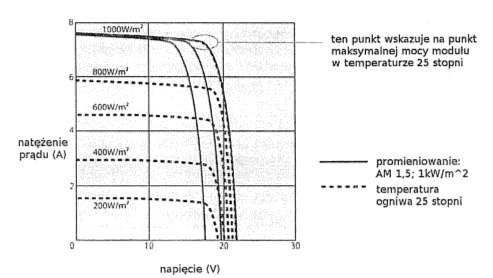
\includegraphics[natwidth=13.05cm,natheight=7.35cm]{media/image10.jpg}
\end{figure}
 
Przyczyną, dlaczego moduły PV mają taką relację między natężeniem i 
napięciem jest charakterystyka ogniw. Są one zrobione z materiału 
półprzewodnikowego, który ma własności diody: 

\begin{itemize}
\item Jeśli do układu podłączymy obciążenie o pomijalnej impedancji, to 
mamy w istocie do czynienia ze zwarciem. Oznacza to, że natężenie będzie 
osiągało maksymalną wartość - \textbf{natężenie zwarcia} Isc. Jest to prąd, który 
umożliwiłby przepływ, jeśli podłączylibyśmy dodatnie i ujemne zaciski 
modułu przy zerowym napięciu (zerowa moc) 
\item Jeśli do układu podłączymy obciążenie o nieskończonej impedancji, 
to w istocie mamy do czynienia z \textbf{obwodem otwartym}. Oznacza to, że żaden 
prąd nie może płynąć, a napięcie na module będzie osiągało maksimum - to 
jest napięcie obwodu otwartego Voc. 
\item Kiedy do układu podłączymy pośrednie obciążenie, moduł PV będzie 
wytwarzał moc, która osiągnie maksimum w punkcie mocy maksymalnej. Ta 
sytuacja pokazana na wykresie powyżej. 
\end{itemize}
 
Diagram powyżej pokazuje, że na ogniwie spada napięcie, jeśli 
temperatura zwiększa się, a natężenie prądu maleje w miarę zmniejszenia 
natężenia promieniowania. Ten efekt jest wspólny dla wszystkich modułów 
krystalicznych. Maksymalną moc wyjściową tego ogniwa jest uzyskiwana w 
punkcie na zakrzywieniu krzywej. 

Inwertery, które są używane systemach podłączanych do sieci 
energetycznej, posiadają układy śledzenia punktu mocy maksymalnej, które 
umożliwiają sterowanie obciążeniem. Pomaga to utrzymać moduły/generatory 
najbliżej jak to możliwe punktu mocy maksymalnej, nawet przy zmianach 
pogody i zmianach zapotrzebowania na elektryczność wewnątrz budynku. 
Dlatego pobór prądu i napięcie układu powinno być blisko punktu mocy 
maksymalnej. 
\section{Moduł 3. Projektowanie systemu PV }

\subsection{Projektowanie systemu fotowoltaicznego}

Rdzeń projektu systemu PV opiera się na dwóch podstawowych zasadach, 
\textbf{połączenia modułów w szereg zwiększa jego zdolność napięciową, a 
konfiguracja równoległa daje większą wydajność prądową}. Jest to 
analogiczne do baterii/akumulatorów, gdzie wymagania związane z 
optymalnym napięciem i natężeniem są ustalone przez konfigurację 
połączenia. 

Napięcia operacyjne większych systemów PV są uzyskiwane poprzez 
połączenie modułów w szeregi w celu zwiększenia napięcia. Wyższe poziomy 
mocy są uzyskiwane przez równoległe łączenie szeregów (o takim samym 
nominalnym napięciu) w celu zwiększenia natężenia. Te własności 
generatora są istotne, ponieważ muszą zostać obliczone, zanim podejmie 
się decyzję co do wielkości inwertera. Typowy system zintegrowany z 
siecią jest zilustrowany poniżej: 

\begin{figure}[h]
\centering
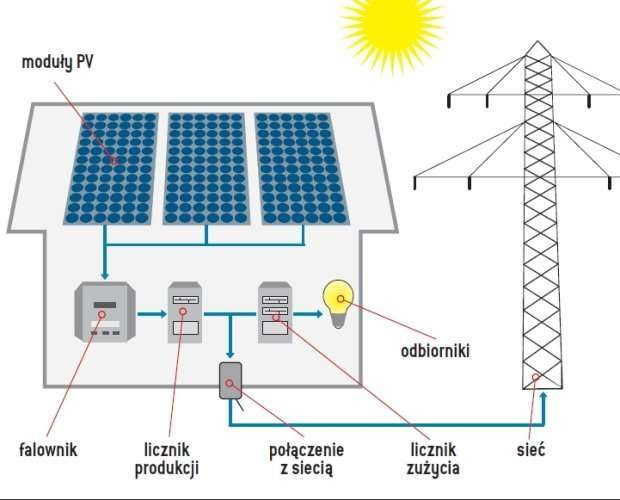
\includegraphics[natwidth=15.90cm,natheight=12.83cm]{media/image11.jpg}
\end{figure}
\subsubsection{Napięcie}

Napięcie i natężenie wyjściowe generatora zależy od konfiguracji i 
połączenia modułów. Jeśli moduły są połączone w szeregi, to spowoduje 
zwiększenie całkowitego napięcia generatora PV, Zauważmy, że istnieją 
dwie wartości napięcia dla danego modułu. Jedno przy warunkach STC i 
drugie w punkcie mocy maksymalnej (MPP). 

Weźmy napięcie modułu przy warunkach STC jako 21,0 V i połączmy 10 
modułów w szereg, co da nam 210 V napięcia na szereg. 

Jeśli napięcie w punkcie MPP przyjmiemy 17 V i znowu moduły będą połączone szeregowo, to uzyskamy napięcie w punkcie mocy maksymalnej równe 170 V na szereg.
Są to proste obliczenia, mnożąc napięcie wyjściowe moduł przez liczbę modułów tworzących szereg. Moduły połączone w szereg nazywa się szeregami (stringami). 

Konfiguracja pojedynczego szeregu (stringa): moduły połączone szeregowo 

\begin{figure}[h]
\centering
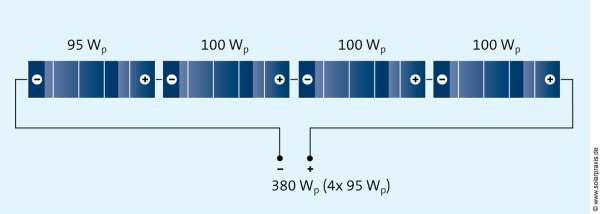
\includegraphics[natwidth=15.92cm,natheight=5.67cm]{media/image12.jpg}
\end{figure}
 
Konfiguracja wielu szeregów (stringów): moduły połączone w szeregi 
(stringi), a te równolegle 

\begin{figure}[h]
\centering
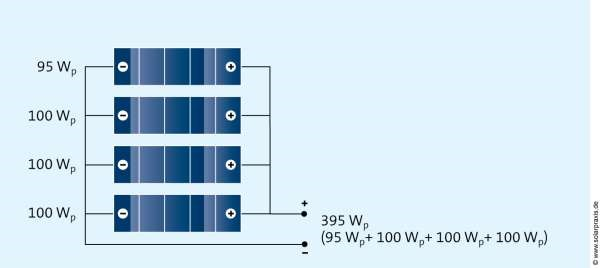
\includegraphics[natwidth=15.92cm,natheight=7.11cm]{media/image13.jpg}
\end{figure}
 

 
\subsubsection{Natężenie}

Taki sam proces jak przed chwilą może być zastosowany do obliczenia 
całkowitego natężenia wyjściowego generatora PV. Istnieją także dwie 
wartości wyjściowe, znowu w warunkach STC i w punkcie MPP. Jeśli wartość 
w warunkach STC wynosi 8,25 A, to tę wartość mnożymy przez liczbę 
szeregów w generatorze. Jeśli są 2 szeregi po 10 modułów w każdym 
(całkowita liczba to 20 modułów), to prąd zwarciowy Izw obliczamy, mnożąc 8,25 
razy 2, i to daje 16,5 A dla całego generatora. Znowu, można obliczyć 
wartość natężenia wyjściowego w punkcie MPP. Jeśli ta wartość wynosiłaby 
16,5 A, to dałoby natężenie wyjściowe w punkcie MPP dla całego 
generatora wielkości 33 A. 


Te obliczenia mogą być przedstawiona jak poniżej: 

\subsubsection{Charakterystyka generatora: }

Napięcie przy otwartym obwodzie (szereg) - liczba modułów x napięcie Voc 
przy STC 

Napięcie w punkcie mocy maksymalnej - liczba modułów x UMP (napięcie 
przy mocy szczytowej) 

Natężenie zwarcia - liczba szeregów x Isc przy STC 

Natężenie w punkcie mocy maksymalnej - liczba szeregów x IMP (natężenie 
przy mocy szczytowej) moc szczytowa = UMP x IMP 


Wartości te używane są do określania wielkości i wymogów technicznych 
inwertera wymaganego przez system i przedstawimy to później w części 4. 

Należy zachować szczególna ostrożność, kiedy wykonuje się połączenie ze 
źródłem trójfazowym, aby zapewnić równomierne obciążanie faz. 

 

\subsection{Przewody i podłączenia}


Przed instalacją systemu PV, o ile to możliwe, powinno zostać wykonane i 
sprawdzone okablowanie. Pozwoli to na skuteczne odseparowanie układu DC 
podczas instalacji generatora. 

Zwykle instalacja wymaga następującego wyposażenia: 

\begin{itemize}
\item Rozdzielnica DC 
\item Przewody do styków + i - od odłącznika DC/skrzynki DC do 
generatora PV 
\item Przewody z odłącznika DC do inwertera 
\end{itemize}
Przewody używane w układzie DC powinny zostać odpowiedni dobrane, aby 
upewnić się, że są odporne na warunki środowiskowe, odpowiednie do 
napięcia i natężenia, przy których będą pracować. Powinno się też 
uwzględniać efekty cieplne będące skutkiem przepływu prądu i światła 
słonecznego. 

\begin{figure}[h]
\centering
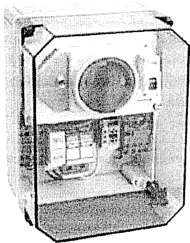
\includegraphics[natwidth=5.03cm,natheight=6.45cm]{media/image14.jpg}
\end{figure}
 


Połączenia/styki/końcówki tych przewodów również powinny zostać poddane 
ocenie parametrów. Odpowiednio dobrane wtyki i gniazda są zwykle 
dopasowane do modułów i szeregów tak, aby uprościć proces instalacji 
generatora PV. Specyficzne złączki DC - odpowiednie do podłączania pod 
napięciem - powinny zapewniać bardzo dobrą ochronę przed porażeniem. 
Pewne własności, na które należy zwracać uwagę to: 

\begin{itemize}
\item Złączki DC muszą posiadać odpowiednie parametry zgodnie ze 
specyfikacją projektu. 
\item Złączki muszą mieć takie same lub większe specyfikacje napięcia i 
natężenia jak przewody, z którymi mają być połączone. 
\item Jeśli złączki mają być dostępne dla nieprzeszkolonego personelu, 
należy umieścić ostrzeżenie . w pobliżu łącznika. Powinno ono brzmieć: 
"Ten wyłącznik nie powinien być rozłączany pod obciążeniem - wyłącz 
najpierw zasilanie AC inwertera." Te wyłączniki mogą zostać uszkodzone 
przez wyładowania łukowe, jeśli zostaną wyłączane pod obciążeniem. 
\item Złączki nie mogą i nie powinny być używane jako sposób 
elektrycznej izolacji DC. 
\item Złączki powinny być bezpieczne w dotyku 
\end{itemize}
 

Wszystkie przewody i złączki muszą być zainstalowane zgodnie z 
odpowiednią normą. Podczas rozważań co do położenia kabli należy wziąć 
pod uwagę wysokie temperatury, które mogą zostać wytworzone przez 
generatory PV, a przewody leżące pod modułami PV powinny mieć 
wytrzymałość minimum 80 \degree C. 

Przewody przechodzące przez dach i ściany powinny być zabezpieczone 
przed mechanicznym uszkodzeniem przez użycie zaprojektowanych do tego 
celu elementów dachowych, przewodów, otworów w dachówkach, a 
uszczelnianie ich za pomocą masy nie jest dopuszczalne. 

Przewody zewnętrzne powinny być odporne na promieniowanie UV, 
wodoodporne, i jest rekomendowane, aby były elastyczne (wielożyłowe), 
aby umożliwić przemieszczanie generatora/modułów spowodowane przez wiatr 
i temperaturę. Aby zminimalizować ryzyko uszkodzenia, drogi przewodów powinny być krótkie na ile to możliwe. 
Kiedy wymagane jest położenie długiego przewodu, dobrą praktyką jest 
opisanie wzdłuż położenia kabli DC informacji: "Niebezpieczeństwo, 
wysokie napięcie (w ciągu dnia) - przewód do generatora PV". Należy 
poinformować personel, który jest odpowiedzialny na konserwację budynku 
o ostatnich zmianach, jakie zostały wykonane. 

Aby uniknąć indukowanych skoków napięcia, na przykład podczas wyładowań 
atmosferycznych, występujących w modułach PV, przewody modułów i 
związanie z nimi kable DC powinny poprowadzone razem (kabel do +, kabel 
do -), o ile to tylko możliwe. Jeśli tak zrobimy, to potencjalne 
utworzenie pętli (indukcyjnej) w instalacji jest zredukowane do minimum, 
co ogranicza wystąpienie indukowanego napięcia. Na obszarach, gdzie 
istnieje wysokie ryzyko uderzenia pioruna, zaleca się wykonanie 
indywidualną osłonę przewodów. 

Należy również starannie rozważyć potencjalne wystąpienie zwarcia 
podczas prowadzenia dodatnich i ujemnych przewodów. Dlatego należy 
zapewnić odpowiednią ochronę, aby uniknąć mechanicznych uszkodzeń. 

\subsection{Diody i bezpieczniki}
 
\subsubsection{Bezpieczniki szeregowe}

W większych instalacjach PV w celu zapobieżenia ryzyka pożaru 
przeciążonych przewodów stosuje się diody i bezpieczniki. Zwyczajowo 
bezpieczniki te są zwane \textbf{bezpiecznikami szeregów}, kiedy są one 
podłączone do głównych przewodów szeregu generatora, zwykle są 
umieszczane w skrzynce przyłączeniowej DC. Bezpieczniki szeregów stosuje 
się w generatorach, które są utworzone z czterech lub więcej szeregów, i 
powinny być dopasowane do obydwu dodatnich i ujemnych przewodów DC dla 
wszystkich szeregów. Bezpieczniki szeregów powinny spełniać następujące 
wymagania: 

\begin{itemize}
\item Bezpieczniki szeregów powinny posiadać parametry odpowiednie do 
pracy w układzie DC przy wartościach występujących w momencie awarii. 
\item Bezpieczniki szeregów powinny posiadać parametry: Voc (STC) x 
liczba modułów w szeregu (M)x 1,15 
\item Bezpieczniki szeregów muszą mieć prąd zadziałania, który jest 
mniejszy niż 2 x Isc (STC), a zdolność przenoszenia natężenia prądu 
przewodu do szeregu wartość mniejszą 
\item Bezpieczniki szeregów można pominąć przy szeregu lub generatorze 
PV, jeśli okablowanie układu jest zdolne przenieść/wytrzymać ciągłe 
obciążenie rzędu 1,25 x Isc (STC) a dowolnym miejscu 
\end{itemize}
 
Układy z trzema lub mniejszą liczbą szeregów w generatorze nie są w 
stanie wytworzyć wystarczających prądów (powodujących 
awarię/uszkodzenie) dających podstawy do użycia bezpiecznika szeregów. 
Stosuje się je jedynie, jeśli przewody z szeregów łączące generator ze 
skrzynką przyłączeniową nie spełniają wymagań dla takich natężeń prądów. 

Należy zaznaczyć, że pominięcie bezpieczników szeregów w przypadku 
generatora składających się z trzech lub mniej szeregów jest 
uzasadnione, jeśli projektant systemu zweryfikował z producentem 
modułów, że są one w stanie przetrwać wsteczny prąd o wartości 2 x 1,15 
x Isc (STC). 

\subsubsection{Diody bocznikujące}

Diody bocznikujące są również używane w układach zintegrowanych z siecią 
w celu zapobieżenia przepływu prądów wstecznych przez równolegle 
połączone moduły. Prądy wsteczne występują tam, gdzie szereg nie był w 
stanie wytworzyć napięcia (na skutek zacienienia albo zwarcia) i tym 
samym dostarczać prądu. Ze względu na to, że szeregi są połączone 
równolegle, to taka sytuacja umożliwia prądowi z innych szeregów 
przechodzić przez niego w przeciwnym kierunku. Ma to szkodliwy wpływ na 
moduły w tym szeregu i może spowodować ich awarię, jeśli moduły nie są 
zaprojektowane tak, aby to wytrzymać. Diody bocznikujące są dopasowane 
do każdego szeregu w przypadku normalnego kierunku przepływu prądu, 
pozwalając w ten sposób przepłynąć przez szereg wypadkowym prądom 
szeregowym, Diody bocznikujące muszą spełniać następujące minimalne 
wymagania napięciowe: 

\begin{itemize}
\item 2 x Voc (STC) x liczba modułów w szeregu 
\end{itemize}
Istnieją jednak pewne wady związane ze stosowaniem diod bocznikujących. 

? Ze względu na to, że diody są połączone szeregowo z szeregami, to 
oznacza, że występuje na nich pewien spadek napięcia. Wynosi on w 
przybliżeniu około 0.7 V. 

\begin{itemize}
\item Uszkodzone diody okazują się problematyczne w szeregach PV, które 
zostały zupełnie uszkodzone, ale uszkodzenie nie zostało wykryte przez 
pewien czas, dlatego zaleca się stosowanie zabezpieczeń nadprądowych 
każdej gałęzi. 
\end{itemize}
Większość systemów PV zintegrowanych z siecią obecnie na ogół jest 
projektowanych bez diod. Standardowe moduły często są w stanie przetrwać 
bez uszkodzenia siedmiokrotnie wystąpienie prądu zwarcia. 

Diody nie są wymagane, jeśli wszystkie poniższe warunki są spełnione: 

\begin{itemize}
\item Jeśli używa się tylko modułów tego samego typu i mamy mniej niż 3 
szeregi (stringi) . Jeśli spełniają one wymagania ochrony Klasy II. 
\item Jeśli moduły posiadają certyfikat, który potwierdza, że są w 
stanie wytrzymać 50\% nominalnego prądu zwarcia płynącego w kierunku 
przeciwnym do normalnego przepływu prądu. 
\item Jeśli napięcie przy obwodzie otwartym nie różni się o więcej niż 
5\% pomiędzy poszczególnymi szeregami 
\end{itemize}


 

\textit{ }\ \ \ \ \textit{ }\ \ \ \ \textit{bezpiecznik }\ \ \ \ 
\textit{ }\ \ \ \ \textit{ }\ \ \ \ \textit{ }\ \ \ \ \textit{ }\ \ 
\ \ \textit{dioda blokująca }

\subsection{Dobór parametrów komponentów DC }


Wszystkie komponenty DC (przewody, wyłączniki, przełączniki, itd.) 
układu muszą posiadać odpowiednie parametry, które zostały obliczone z 
uwzględnieniem maksymalnego napięcia i natężenia generatora PV. Należy 
uwzględnić napięcia i natężenia szeregowo/równolegle połączonych modułów 
tworzących generator PV, a także indywidualne charakterystyki wyjściowe 
modułów. Dwie wielkości, które należy rozważyć to Voc i Isc przy 
warunkach STC. Jak powiedziano wcześniej, warunki STC nie występują 
bardzo często (w Wielkiej Brytanii), ale wartości tych należy użyć w 
obliczeniach, ponieważ zawsze istnienie możliwość, że takie warunki mogą 
się pojawić i nasz układ musi być w stanie wtedy funkcjonować. 

Istnieje wiele czynników, które mogą zostać dopasowane do warunków 
występujących w Wielkiej Brytanii w przypadku modułów mono- i 
polikrystalicznych. 

Wszystkie komponenty DC muszą mieć parametry co najmniej: 

Napięcie: Voc STC x 1,15 Natężenie: Isc STC x 1,25 

Kiedy wykorzystujemy moduły różnych typów, wszystkie komponenty DC 
powinny mieć minimalne parametry określone następująco: 

Szczegółowe obliczenia dla najgorszego przypadku dla Voc i Isc. Te 
wartości powinny zostać 
obliczone dla danych producenta 
dla zakresu temperatur od -10 do 
80 \degree C i poziomu promieniowania 
aż do 1250 W  m2. 
Główne przewody DC (od i do całego generatora) powinny mieć minimum 
następujące parametry: 

Napięcie: Votw STC x M x 1,15 (gdzie M jest liczbą szeregów połączonych 
modułów) Natężenie: Izw 

STC xNx 1,25 (gdzie N oznacza liczbę równolegle połączonych szeregów) 

Przewody DC w szeregach powinny mieć parametry jak poniżej: Generator PV 
bez bezpieczników szeregowych: 

 

Napięcie: Votw STC x M x 1,15 (M liczba modułów połączonych w szeregu) 

Natężenie: Izw STC x 1,25 

\underline{Generator PV bez bezpieczników szeregów:} 

Napięcie: V$_{oc}$ STC x M x 1.15 (gdzie M jest liczbą modułów 
połączonych w szeregu) Natężenie: I$_{sc}$ STC x (N-l) x 1.25 (gdzie 
N jest liczbą równolegle połączonych szeregów) 

W przypadku gdy nie ma bezpieczników szeregów, należy przy obliczeniach 
parametrów uwzględnić mnożnik (N-1). Z teorii wynika, że maksymalny prąd 
płynący przez przewód szeregowy, który spowodowałby uszkodzenie, 
wynosiłby (N-1) x lsc, gdzie N to liczba równolegle połączonych 
szeregów. Dla mniejszych systemów należy się upewnić, że przewody w 
szeregach posiadają parametry, które pozwalają bezpiecznie płynąć 
maksymalnemu prądowi powodującemu uszkodzenie. Taka metoda obliczeń 
opiera się na przeszacowaniu parametrów przewodów w taki sposób, że prąd 
powodujący uszkodzenie jest dopasowany i chociaż to nie spowoduje 
uniknięcia awarii, to jednak zapobiegnie ryzyku powstania pożaru z 
powodu przeciążenia przewodów. 

Przewody, które są poprowadzone pod generatorem PV powinny wytrzymywać 
temperaturę minimum 80\degree C. 

Okablowanie DC powinno także zostać wybrane tak, aby zminimalizować 
ryzyko doziemienia czy zwarcia. Można to osiągnąć poprzez następującą 
metodę okablowania: 

\begin{itemize}
\item Przewód jednożyłowy - podwójnie izolowany 
\item Przewód jednożyłowy prowadzony w odpowiednich 
rynnach/korytkach/listwach 
\item Przewód zbrojony SWA z osnową stalową - zwykle odpowiedni tylko 
dla głównego okablowania DC. 
\end{itemize}
Wszystkie przewody powinny mieć dobrane rozmiary zapewniające spadek 
napięcia mniejszy niż 3\% przy warunkach STC na odcinku pomiędzy 
generatorem PV a inwerterem. Wszystkie zewnętrzne kable powinny być 
odporne na działanie promieniowania UV, wodoodporne i giętkie.  

\subsection{Ocena parametrów komponentów AC }

Przewody AC powinny posiadać odpowiednie parametry i być zainstalowane w 
zgodzie z odpowiednią normą. Zasilanie AC z inwertera powinno być 
wprowadzone do gniazdka w odbiorniku z użyciem właściwego wyłącznika 
instalacyjnego (wyłącznik nadprądowy), który powinien zostać odpowiednio 
dobrany do typu i wyjścia inwertera. 
 

\subsubsection{Rozłączniki generatora - rozłącznik AC i DC }


Ze względu na naturę systemu PV, system należy wyposażyć w odłączniki AC 
i DC. Zapewniają one sposób ręcznego odseparowania elektrycznego całego 
generatora PV. Odłączniki te są wymagane podczas instalacji systemu, a 
następnie przy pracach konserwacyjnych i serwisowych. Odłączniki AC i DC 
powinny być umiejscowione w pobliżu inwertera. 

W przypadku odłączników DC należy przestrzegać: 

\begin{itemize}
\item Odłącznik DC musi być dwubiegunowy - aby elektrycznie odizolować 
zarówno przewody plus i minus generatora PV, 
\item Odłącznik musi posiadać parametry do pracy w zakresie systemu DC. 
\item Dla odłączenia głównego systemu DC rekomendowany jest odłącznik 
obciążenia. 
\item Jeśli nie wybierzemy odłącznika obciążenia, to wybrany model 
powinien posiadać blokadą. 
\item Gdy blokada nie jest dostępna, i nie wybrano odłącznika 
obciążenia, to ten fakt powinien być wyraźnie oznakowany: "\,Ten 
odłącznik nie funkcjonuje pod obciążeniem - odłącz najpierw zasilanie 
zmiennoprądowe inwertera' '. Taka opcja nie jest preferowana. 
\item Odłącznik DC musi posiadać parametry odpowiadające maksymalnym 
występującemu napięciu i natężeniu. Te powinny odpowiadać napięciu przy 
obwodzie otwartym w temperaturze -10 o C i natężeniu prądu zwarcia przy 
warunkach STC. 
\item Odłącznik DC powinien być oznakowany jako "\,Główny odłącznik 
generatora PV", z wyraźnie oznakowanymi pozycjami włączenia i 
odłączenia. Obudowy odłączników powinny również zawierać ostrzeżenie: 
"\, Niebezpieczeństwo, występują części p od napięciem w ciągu dnia." 
Wszystkie etykiety powinny być wyraźne, łatwo widoczne, dobrze 
umocowane. 
\end{itemize}
 

Nie należy stosować odłączników AC o takich samych parametrach w miejsce 
odłączników DC. Odłączanie obwodów AC jest mniej wymagające ze względu 
na to, że wartość napięcia przechodzi przez punkt 0V wiele razy w ciągu 
sekundy. 

Zaleca się przy wyborze odłącznika DC, aby wybrać typ odcinający 
obciążenie. Nawet nieodcinające obciążenia wyłączniki stanowią tańszą 
alternatywę. Nie mogą one jednak być przełączane bez uprzedniego 
wyłączenia inwertera za pomocą odłącznika AC. W pobliżu takiego 
odłącznika DC należy umieścić odpowiednią tabliczkę, aby zapewnić 
wykonanie takiej procedury. Uszkodzenie może być spowodowane przez 
przypadkowe wyłączenie podczas pracy pod obciążeniem i chociaż może to 
być niewidoczne, to może poważnie zmniejszyć wydajność i bezpieczeństwo 
użytkowania wyłącznika. 

\begin{figure}[h]
\centering
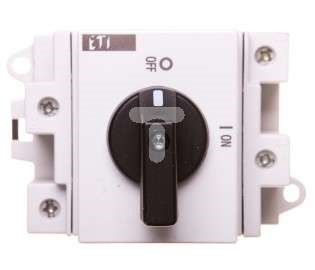
\includegraphics[natwidth=7.57cm,natheight=6.48cm]{media/image23.jpg}
\end{figure} 

W przypadku odłączników AC należy przestrzegać: 

Zgodnie z normą powinny się występować 2 odłączniki pomiędzy 
inwerterem i punktem podłączenia zasilania. Jeden powinien zostać 
zainstalowany w pobliżu inwertera, a drugi w pobliżu odbiornika energii. Jeśli obydwa miałyby się znajdować w tym samym pomieszczeniu, wymagany jest tylko jeden. 

\begin{itemize}
\item Odłączniki powinny odłączać wszystkie przewody pod napięciem i 
przewody neutralne (wielobiegunowe) 
\item Powinny mieć zrozumiałe oznaczenia pozycji WŁĄCZONE i WYŁĄCZONE 
oraz etykietę \underline{,,} \underline{System PV - wyłącznik 
awaryjny.''} 
\item Odłącznik w pobliżu odbiornika energii powinien mieć możliwość 
blokady tylko w pozycji WYŁĄCZONE i powinien być łatwo dostępny. Oznacza 
to, że odłącznik NIE MOŻE mieć blokady w pozycji WŁĄCZONE. 
\item W punkcie zamontowania każdego odłącznika AC, sieć publiczną 
powinno się uważać za źródło, 
\end{itemize}
a instalację PV należy uznać za obciążenie. 

\begin{center}Wymagania odnośnie odłączników AC są częścią odpowiednich 
norm. \end{center}

\begin{figure}[h]
\centering
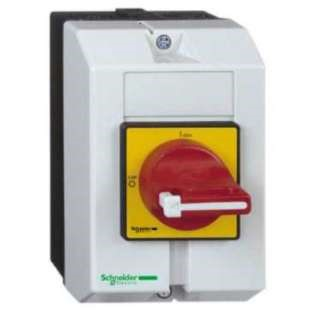
\includegraphics[natwidth=8.40cm,natheight=8.40cm]{media/image24.jpg}
\end{figure}
 

\textbf{ }

Skrzynki przyłączeniowe 

Skrzynki przyłączeniowe DC mają zastosowanie w przypadku, gdy istnieje 
więcej niż jeden szereg (string). Skrzynka przyłączeniowa jest punktem, 
gdzie szeregi są łączone równolegle jeden z drugim. Jest to też punkt, w 
którym podłącza się bezpieczniki szeregowe (jeśli się je stosuje). 

Skrzynki przyłączeniowe DC powinny zawierać: 

\begin{itemize}
\item Skrzynki przyłączeniowe DC powinny być oznakowane jako ,, Skrzynka 
przyłączeniowa generatora PV " a także: "\, Niebezpieczeństwo! Zawiera 
elementy pod napięciem w ciągu dnia." Wszystkie etykiety powinny być 
wyraĽne, łatwo widoczne, dobrze umocowane i długotrwałe. 
\item Rekomenduje się, aby istniały sposoby odłączania i odseparowania 
poszczególnych szeregów od generatora PV, które można bezpiecznie 
obsługiwać, gdy są one pod napięciem. Można to osiągnąć przez 
zastosowanie odpowiednich wymiennych zespołów bezpieczników wewnątrz 
skrzynki przyłączeniowej lub innych ruchomych łącz. Nie powinno się 
wykonywać takiego odłączania, jeśli system jest pod obciążeniem. 
\end{itemize}
Konstrukcja skrzynek przyłączeniowych DC również musi uwzględniać poziom 
oferowanej ochrony przed zwarciem. Rekomenduje się, że ochrona przed 
zwarciem była osiągana przez: 

\begin{itemize}
\item Obudowy z materiałów były wykonane całkowicie nieprzewodzących. 
\item Szyny montażowe dla biegunów + i - były adekwatnie 
odseparowane/oddzielone przez zastosowanie odpowiednich płyt izolujących 
albo odseparowanie przez użycie osobnych skrzynek dla biegunów + i . 
Przewody i układ zacisków były taki, aby zwarcie podczas instalacji lub 
prac serwisowych było wyjątkowo mato prawdopodobne. 
\item Gdy mają być połączone do skrzynki przyłączeniowej tylko dwa 
szeregi - alternatywą był łącznik szeregów. Jeden pokazany tutaj jest 
łącznikiem dla złączek MC4, które po prostu podłącza się z szeregów, a 
potem pojedynczą złączkę do inwertera. 
\end{itemize}
 

\begin{figure}[h]
\centering
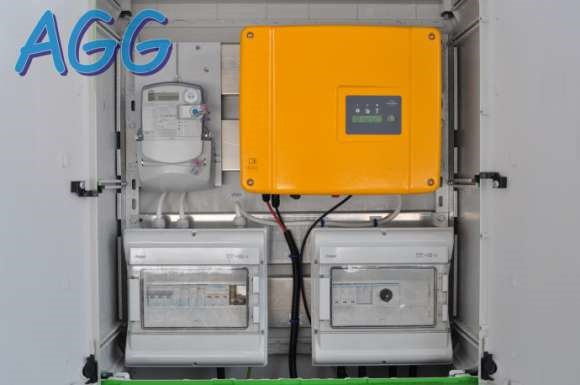
\includegraphics[natwidth=15.35cm,natheight=10.20cm]{media/image25.jpg}
\end{figure}
 

 

Bezpieczne odizolowanie 

Wszystkie panele PV są pod napięciem od momentu wytworzenia i z tego 
powodu powinny być uznane jako faktycznie wytwarzające elektryczność 
przez cały czas. Normy stwierdzają, że "\,Osprzęt PV po stronie DC 
powinien być uznany jako będący pod napięciem, nawet jeśli system PV 
jest odłączony ze strony AC." Mając to na uwadze, przypisujemy 
zwiększoną wagę procesowi bezpiecznego odizolowania, pracy w warunkach 
pod napięciem zgodnie z przepisami BHP oraz podzieleniu procesu 
instalacji na etapy. Należy z tego powodu starannie przestrzegać 
sekwencjonowania procesu instalacji, gdyż zapewnia to, że podczas 
żadnego etapu instalacji 

instalatorzy nie będą wystawieni na działanie niebezpiecznych napięć DC. 
Na przykład, montowanie zacisków i podłączanie powinno być wykonywane 
przy wyłączonym napięciu, a sekwencjonowanie zadań zapewnia ochronę 
przed będącymi pod napięciem końcówkami DC i złączami. Proces podziału 
na etapy musi być odzwierciedlony we wszelkiej dokumentacji oceny 
ryzyka. 

 

Bezpieczne odizolowanie jest kluczowym procesem przy wykonywaniu każdej 
pracy związanej z elektrycznością i solarne systemy fotowoltaiczne nie 
są tu żadnym wyjątkiem. Ze względu na unikalną naturę wytwarzania 
elektryczności, instalatorzy powinni mieć większą świadomość 
niebezpieczeństwa prac związanych z podłączaniem i konserwacją systemów 
PV. Systemy PV są nietypowe pod tym względem, że nie mogą zostać 
wyłączone, dlatego każde złącze pozostaje pod napięciem cały czas w 
ciągu dnia. Pamiętając o tym, bezpieczne odizolowanie powinno być 
stosowane cały czas, aby zapobiec porażeniu i poparzeniu prądem. 

Dobrą praktyką jest instalowanie modułów/generatorów PV jako ostatnich 
elementów układu w celu redukcji ryzyka opisanego powyżej. Jeśli to nie 
jest możliwe, to przykrycie arkuszem i zaciemnienie generatora nie jest 
uznawane za bezpieczny sposób odizolowania. Powinno się zastosować 
poniższe informacje i procedury. 

Należy użyć odłączników DC i AC odpowiednio dobranych do systemu PV a 
celu zapewnienia bezpiecznego odizolowania. 

W celu odizolowania układu DC odłącznik DC, umieszczony w pobliżu 
inwertera, powinien być wyłączony (tylko jeśli ma możliwość odcięcia 
obciążenia) w celu odcięcia zasilania DC, które jest podpięte do 
inwertera. W większości wypadków, odłącznik DC nie ma funkcji 
zablokowanie go w pozycji wyłączonej, więc musimy mieć zdejmowalną 
dĽwignię, którą można przechowywać w osobnym miejscu (zamykanej 
skrzynce), która powinna być dostępna od osoby wykonującej odizolowanie. 
W celu odłączenia układu 'AC odłącznik AC, umiejscowiony w pobliżu 
odbiornika energii, powinien być wyłączony. Odłącznik AC powinien być 
zablokowany w pozycji wyłączony przy użyciu odpowiedniej blokady. 

Powinno się wyeksponować informacje ostrzegawcze we wszystkich miejscach 
gdzie można dokonać odizolowania, dostarczając informacji o osobie, 
która wykonała odizolowanie i jak się z nią skontaktować. 

W miejscach gdzie jest wykonywana praca związana z instalacją, należy 
stosować zestaw odpowiednich próbników albo dwustanowe wskaźniki 
napięcia. Kiedy wskaźniki pokazują, że napięcie systemu AC jest 
wyłączone, następująca przeprowadzić następującą procedurę: 

\begin{itemize}
\item WskaĽniki napięcia powinny sprawdzone na znanym testowym źródle 
pod napięciem. 
\item Sprawdzić napięcie pomiędzy stykami: 
\end{itemize}
 uziemionym i fazowym, neutralnym i fazowym, uziemionym i neutralnym. . 
Ponownie należy sprawdzić wskaĽniki napięcia na znanym testowym Ľródle 
pod napięciem. Aby przetestować nie będącą pod napięciem część DC 
układu, należy przeprowadzić następującą procedurę: 

 

WskaĽniki napięcia powinny być sprawdzone na znanym testowym Ľródle pod 
napięciem. 

? Sprawdzić napięcie między stykami: 

uziemionym i plusem, minusem i plusem, uziemionym i minusem. 

Ponownie sprawdzić wskaĽniki napięcia na testowym Ľródle pod napięciem. 



\section{Moduł 4. Montaż systemu PV }

\subsection{Podstawowe zasady projektowania}
  

Przed rozpoczęciem projektowania solarnego generatora fotowoltaicznej, 
należy zebrać charakterystyki budynku w celu określenia, jaki będzie w 
tym miejscu odpowiedni system PV, Należy uwzględnić: 

\begin{itemize}
\item Czy budynek posiada odpowiednią konstrukcje dachu/fasady, która 
jest w stanie wytrzymać obciążenie generatora PV? Rekomenduje się 
przeprowadzenie badania zdolności nośnej konstrukcji przed wykonaniem 
prac projektowych. 
\item Czy budynek posiada odpowiednio dużo miejsca na dachu/fasadzie o 
odpowiednim nachyleniu (zwykle między 30 a 40 stopni), aby była możliwa instalacja generatora PV? 
\end{itemize}

Jest to istotny aspekt wymaganych informacji związanych z 
instalacją, ponieważ to decyduje czy instalacja PV będzie efektywna pod 
względem kosztów dla klienta i bezpośrednio wpływa na liczbę 
modułów/parametry napromieniowania słonecznego, które determinują 
wartości wyjściowe generatora. 

\begin{itemize}
\item Czy budynek posiada dach/fasadę skierowaną ku południu, do której 
będzie można zamontować generator PV? Jeśli budynek nie ma takiego 
dachu/takiej fasady, to spowoduje, że niedostateczna ilość 
promieniowania słonecznego, na które jest wystawiony generator, 
zredukuje parametr/ na wyjściu generatora. 
\item Jakie materiały zostały użyte do zbudowania budynku i czy solarny 
generator PV może być w odpowiedni sposób przymocowany do tych 
materiałów? Jeśli, na przykład, pochylony dach ma wiązary dachowe, to w 
tej sytuacji jest możliwe zamontowanie haków i systemu uchwytów, podczas 
gdy inny system - np. posiadający płaski betonowy dach - wymagałby 
zastosowania pomocniczej konstrukcji ramowej. Mogą wystąpić również 
pewne okoliczności, w których gdy generatora PV nie można zamontować.
\end{itemize}
 

\subsection{Planowanie instalacji }


Rozpoczęcie planowania pracy w zaciszu domowym albo za biurkiem, zanim 
przybędzie się na miejsce, może okazać się pożyteczną aktywnością. 
Opierając się na informacjach z inspekcji o miejscu instalacji i 
specyfikacji systemu, powinniśmy być zdolni wykonać następujące 
rozplanowanie zasobów: 

\begin{itemize}
\item Określ harmonogram prac instalacji (włączając poszczególne 
zadania). 
\item Sporządź listę wszystkich części: tych, które są dostępne i tych, 
które trzeba jeszcze zdobyć; sprawdź czy dostarczony sprzęt jest 
kompletny i nieuszkodzony. 
\item Sporządź listę dokumentacji, narzędzi i wyposażenia włączając 
sprzęt do zapewnienia bezpieczeństwa i podesty/rusztowania wymagane do 
konkretnej pracy. Określ, jakie umiejętności, ile ludzi, ile godzin 
prawdopodobnie będziesz potrzebować. Zaplanuj harmonogramy pracy. 
\item Sporządź listę wszystkich wstępnych prac, które trzeba wykonać 
\end{itemize}
 

\subsection{Podsumowanie sekwencjonowania zadań na miejscu instalacji }

Całe okablowanie PV powinno być, o ile to możliwe, ukończone przed 
montażem generatora PV. 

Umożliwi to skuteczne odizolowanie elektryczne układu DC) dzięki 
odłącznikowi DC i wtykom modułu PV) podczas instalacji generatora, i 
efektywne elektryczne odizolowanie generatora PV podczas montażu 
inwertera. Zwykle wymaga to montażu: 

\begin{itemize}
\item Odłączników DC i rozdzielnic DC 
\item Przewodów plus i minus - z odłącznika DC/skrzynki przyłączeniowej 
do obydwu końców generatora/szeregu PV 
\item Głównych przewodów generatora PV od odłącznika DC do inwertera. 
\end{itemize}
Czynności te powinny być wykonane w taki sposób, aby nigdy nie było 
konieczne, by instalator nie musiał pracować w żadnej sytuacji, w której 
jednocześnie byłyby dostępne części plus i minus szeregu PV, które są 
pod napięciem. Podczas gdy instalator będzie zajmował się - podczas 
kolejnych etapów instalacji - przewodami pod napięciem, nie będzie 
możliwości porażenia prądem z częściowo zainstalowanego szeregu PV, 
ponieważ obwód jest przerwany na odłączniku DC. Maksymalne napięcie 
powodujące porażenie elektryczne, które występuje w układzie, jest 
napięciem pojedynczego modułu PV. W przypadkach, gdy nie ma możliwości 
wcześniejszego zainstalowania odłącznika DC (np. nowy projekt, gdzie 
generator PV jest instalowany zanim ukończy się pomieszczenie), 
końcówki/wtyki przewodów powinny być tymczasowo umieszczone w skrzynce 
izolacyjnej i odpowiednio oznaczone. 

\subsubsection{Roboty na dachu}
Aby do minimum ograniczyć zakłócenia w 
funkcjonowaniu gospodarstwa domowego, i zredukować możliwe opóźnienia 
związane z niekorzystną pogodą, wszystkie prace zewnętrzne włączając 
dostęp do dachu i roboty dachowe powinny być wykonane w pierwszej 
kolejności. Może to sprawić problemy w przypadku, gdy generator PV jest 
pod napięciem i wytwarza energię elektryczną. W tej sytuacji powinien 
zostać on przechowany w opakowaniu na posesji z okablowaniem DC gotowym 
do podłączenia, gdy tylko zostanie ukończona pozostała część instalacji. 
Jeśli to nie byłoby praktyczne, to prace na dachu i instalacja 
generatora powinna być ostatnim zadaniem do wykonania. 

 

\subsubsection{Roboty wewnątrz }
Roboty wewnątrz zwykle mogą być wykonywane w tym samym czasie co prace 
na dachu, jeśli na to pozwalają tylko względy bezpieczeństwa. Może się 
zdarzyć, że pogoda może czasem zmusić do wykonania w pierwszej 
kolejności robót wewnątrz budynku. 

Zwykle to inwerter, odłączniki DC i AC oraz licznik energii są 
instalowane jako pierwsze, a potem kładzie się przewody połączeniowe 
między nimi. 

 

\subsubsection{Potrzebne narzędzia}

Cały elektryczny osprzęt w miejscu instalacji powinien działać przy 
napięciu poniżej 36V DC dzięki transformatorowi sieciowemu albo 
generatorowi zasilania. Nie należy używać sprzętu elektrycznego w 
przypadku występowania wilgoci. Wszystkie bezprzewodowe urządzenia 
elektryczne powinny być objęte testem potwierdzającym możliwość pracy na 
zewnątrz. 

 

\subsubsection{Lista potrzebnych narzędzi:}

\begin{itemize}
\item drabina ze stopniami 
\item drabina 3 x 3.5m - po rozłożeniu 7,2m 
\item drabina dachowa 4,3m - po rozłożeniu 7,6m 
\item drabina dachowa 2,9m - po rozłożeniu 4,6m 
\item uprząż + 1,5 linka 
\item zacisk ręczny 
\item lina (10-12 mm gruba x 30m długa) 
\item zabezpieczenie liny, które można przymocować do dachu, chroniąca 
linę przy krawędzi dachu 
\item pas narzędziowy 
\item nieścieralny pisak 
\item kreda (do zaznaczania) 
\item podkładka do klęczenia (około l,2m x 0,5m) 
\item arkusze przeciwpyłowe (około 20m) 
\item taśma miernicza (5m) 
\item pistolet do pianki uszczelniającej 
\item klucze oczkowe 10,13,17, 19mm 
\item klucz nastawny 12" (do 34mm) 
\item klucz nasadowy 10,13, 17,19 mm 
\item śrubokręty 
\item nożyk + ostrza 
\item piłka do drewna 
\item szczotka druciana 
\item przenośna poziomica 
\item pitka do metalu (300mm + brzeszczoty) 
\item młotek ciesielski 
\item 4,5" szlifierka z tarczami do ciecia (dachówek) 
\item wiertarka 
\item uszczelniacz silikonowy . taśma izolacyjna w różnych kolorach do 
zaznaczania przewodów fazowych i neutralnych 
\item nożyce do przewodów 
\item szczypce 
\item miernik do wykonywania pomiarów 
\item przewody AC i DC zaciskarka 
\item lampy 
\item poręczna latarka 
\item termometr cyfrowy 
\item kompas o płaskiej krawędzi lub GPS 
\item kombinezon 
\item maska przeciwpyłowa 
\item buty ochronne 
\item rękawiczki z izolacją odporne na działanie czynników chemicznych 
\item kask 
\item kurtkę przeciwdeszczową 
\item chustki i szmaty 
\item zestaw do pierwszej pomocy 
\end{itemize}
Przez cały czas instalacji wymagana jest obecność co najmniej 2 
kompetentnych osób. Wszystkie stosowane materiały powinny być używane 
zgodnie z instrukcją producenta. 

 

\subsubsection{Droga na miejsce montażu i powrót }


Przed wyruszeniem przeprowadź ocenę ryzyka związanego z pogodą. Lądując 
samochód, zanotuj wszystkie stosowne numery seryjne urządzeń. Jeśli 
droga na miejsce instalacji jest długa, to rozważ: bezpieczeństwo, 
zmęczenie, przerwy podczas transportu, wszystkie towary i urządzenia 
powinny być bezpiecznie składowane w pojazdach w celu minimalizacji 
możliwości uszkodzenia albo kradzieży. 

 

\subsubsection{Przybycie na miejsce }


Sprawdź czy wszystkie towary i urządzenia są nieuszkodzone 

\begin{itemize}
\item Zabezpiecz samochód 
\item Na początku przedstaw się klientowi, przywitaj się, i powiedz, że 
dokonasz ponownej oceny miejsca instalacji, i że planujesz się z nim 
spotkać ponownie, zanim rozpoczniesz pracę 
\item Dokonaj ponownej oceny ryzyka związanego z warunkami pogodowymi, 
odłóż prace na dachu, jeśli miałyby być niebezpieczne 
\item Oceń warunki w miejscu instalacji, zwracając uwagę na wszystkie 
aspekty, włączając zdrowie i bezpieczeństwo 
\item Oceń stan dachu i szczegółowo go sfotografuj, uświadom klienta o 
uszkodzeniach takich jak pęknięte dachówki - zanim rozpoczniesz pracę 
\item Sprawdź wykonalność instalacji i dokładność wszystkich 
wcześniejszych \textbf{\textit{przeglądów / pomiarów /planów}} 
włączając zaproponowany sposób podniesienia paneli, ulokowanie i 
orientację używając kompasu z korektą dewiacji magnetycznej 
\item Sprawdź warunki wewnątrz budynku, aby określić czy poddasze jest 
bezpieczne i wolne od przeszkód 
\item Sprawdź wszystkie zamierzone miejsca położenia przewodów oraz 
przeszkody i trudności, jakie mogą się pojawić 
\item Dokonaj krytycznej oceny rusztowania/podestów umożliwiających 
dostęp do dachu (jeśli zostały dostarczone) 
\item Jeśli warunki atmosferyczne w miejscu instalacji są odpowiednie w 
ciągu dnia, krótko poinformuj mieszkańców, co i kiedy będzie wykonywane, 
określając przewidywaną skalę czasową oraz przekaż informacje dotyczące 
implikacji tych robót dla bezpieczeństwa i zdrowia mieszkańców 
\end{itemize}
 

\subsubsection{Rusztowanie }


Jest istotne, aby miejsce gdzie odbywa się praca nie spowodowało upadku 
z wysokości większej niż 2m. Implikacją tego jest, aby szerokość 
jakiegokolwiek rusztowania zwykle rozciągała się znacząco więcej niż 
szerokość jakiegokolwiek generatora PV. Najbardziej bezpieczne, ale też 
najbardziej czasochłonne rusztowania do zbudowania, to tradycyjne 
stalowe rusztowania warszawskie. Na rynku są również dostępne 
specjalistyczne, przenośne, lekkie rusztowania aluminiowe. 

 

\subsubsection{Prace na dachu }
Wymagane kompetencje muszą obejmować bezpieczną pracę na wysokości i 
szkolenia na dachu. Potrzebne są dwie osoby. PotwierdĽ z klientem 
lokalizację generatora. Zdecyduj dokładnie, w którym miejscu na dachu 
zostanie zamontowana instalacja. Jeśli jest to konieczne, wykonaj 
potrzebne otwory w uchwytach dachowych jeszcze przed wejściem na dach. 

 

\subsubsection{Mocowanie generatora do krokwi }


Sprawdź czy krokwie są wystarczająco mocne. Jeśli nie jesteś pewien, 
poproś inżyniera budowlanego, aby wykonał dla Ciebie obliczenia, Na ogół 
jeśli krokiew ma być podparciem dla generatora PV, powinna mieć 
powierzchnię przekroju poprzecznego przynajmniej 7500 mm2. Jeśli żadna 
krokiew nie spełnia tego wymagania, to wtedy albo dodaj prostopadłą 
belkę pomiędzy dwiema krokwiami, albo wzmocnij krokiew tak, aby 
spełniała to wymaganie. 

Aby zapobiec ryzyku uszkodzenia konstrukcji dachu na skutek pęknięcie 
krokwi, wąskie krokwie powinny być wzmocnione. Alternatywnie należy 
zamocować pomiędzy krokwiami rozpory grubości co najmniej l00 mm, 
używając wsporników albo mocnych śrub do przytwierdzenia ich do krokwi. 
Zanim zostanie przytwierdzona rozpora należy w dachu wywiercić otwór 
zewnętrzny, a następnie dopasować do niego rozporę (czynność, do której 
potrzebne są dwie osoby). 


Podczas oceny pokryć dachowych, należy ustanowić wytyczne, kiedy 
wymagane roboty dachowe możemy wykonać we własnym zakresie, a kiedy są 
poza kompetencjami instalatorów i wtedy najlepiej jest je zostawić 
dekarzom. 
 

Łupki (rodzaj kamiennej dachówki) powinny być ułożone jak wątki ceglane, 
zachodzić na siebie na podwójną zakładkę, aby uniknąć wnikania wody. Są 
lżejsze (jeśli bierzemy pod uwagę ciężar przypadający ma metr 
kwadratowy) niż zwykłe dachówki. Łupki nie posiadają występów 
ułatwiających pozycjonowanie na spodniej stronie, więc każdy łupek musi 
być dopasowany indywidualnie i przymocowany do połaci dachowej. Z tego 
powodu wykonanie pokrycia dachowego z łupków jest bardziej czasochłonne 
niż z dachówek. Łupki są zwykle odpowiednie na dachy skośne o nachyleniu 
23 stopnie lub więcej. Większe łupki mogą zostać zastosowane nawet dla 
mniejszych nachyleń. 

Alternatywami dla łupków naturalnych są łupki wykonane ze sztucznych 
materiałów. Niektóre są lżejsze, a większość tańsza. 
 
Dachówki na pióro i wpust są zazwyczaj wykonane z betonu. Posiadają 
profil, który umożliwia dachówkom zachodzenie jedna na drugą, dając 
lepszą ochronę przed wnikaniem wody. Ich typowy rozmiar to 380mm x 
230mm, a efektywna szerokość to 200mm (tj. 30mm na zakładkę). Zwykle są 
układane liniami prostymi w górę dachu na pojedynczą zakładkę. Są 
cięższe (jeśli brać pod uwagę ciężar przypadający na metr kwadratowy) 
niż łupki, ale lżejsze niż zwykłe dachówki. Występy na spodniej stronie 
ułatwiające pozycjonowanie są wykorzystywane do przytwierdzania ich do 
połaci dachowej. Są odpowiednie na dachy skośne o nachyleniu 23 stopnie 
lub więcej. 


Zwykłe dachówki były tradycyjnie wytwarzane z gliny, ale obecnie robi 
się je z betonu i mają zazwyczaj wymiary około 265mm x 165mm. Muszą być 
układane jak wątki ceglane na podwójną zakładkę, aby uniknąć wnikania 
wody po bokach. Ze względu na podwójną zakładkę, są cięższe zarówno niż 
łupki, jak i dachówki na pióro i wpust. Występy ułatwiające 
pozycjonowanie są wykorzystywane do mocowania ich do połaci dachowej. Są 
odpowiednie na dachy skośne o nachyleniu 35 stopni lub więcej. 

Jeśli chodzi o łatwość montażu, dachówka holenderska jest na ogół 
przeznaczona do układania na jedną zakładkę i mocuje się ją jedynie na 
grzbiecie, kalenicy i okapach oraz wokół otworów dachowych. Umożliwia 
ona łatwy montaż uchwytów dachowych, ponieważ mogą one zostać wpuszczone 
pod dachówkę znajdującą się powyżej lub ostrożnie usunięte. Rząd 
podniesionych dachówek może zostać użyty do tego, aby dekarze mogli 
przemieścić dach, o ile uważają, aby nie uszkodzić znajdującej się pod 
spodem izolacji. Jednak, łupki układane na podwójną zakładkę są 
trudniejsze w montażu, ponieważ są one wszystkie przytwierdzane na dachu 
i tworzą bardziej delikatne pokrycie dachowe, które może ulec pęknięciu, 
gdy chodzi się po nim, szczególnie w przypadku łupków naturalnych, które 
zwietrzały na starym dachu. 

Izolacja/papa jest materiałem znajdującym się pomiędzy spodem 
łupków/dachówek a szkieletem konstrukcji dachu zapewniającym dodatkowa 
ochronę i barierę wodoodporną. Tradycyjnie jest wykonana z warstwy 
bitumicznej osadzonej na silnej tkanej osnowie. Osnowa jest podatna na 
pękanie na skutek starzenia się i na gnicie, w miejscach gdzie jest 
wystawiona na działanie promieni słonecznych. Nowoczesne alternatywy są 
na ogół lżejsze i wytrzymalsze. 

Dachy płaskie są normalnie pokryte systemem dwóch lub trzech warstw papy 
- na gorąco, przy użyciu płomienia palnika. Zamiast tradycyjnej papy 
asfaltowej można użyć innych materiałów np. bazujących na polimerach 
oferujących lepsze parametry. Wierzchnią powierzchnię można pokryć 
zapobiegającą pękaniu posypką albo pomalować warstwą odbijającą 
promieniowanie słoneczne. Każde naruszenie chociaż jednej z trzech 
warstw musi być na nowo uszczelnione, aby utrzymać wodoodporność. 

\subsubsection{Sekwencja prac na dachu}
  

Całe okablowanie DC powinno być ukończone przed montażem solarnego 
generatora PV. Umożliwi to skuteczne elektryczne odseparowanie układu DC 
(dzięki odłącznikowi DC i złączkom przewodów modułu PV) podczas montażu 
generatora oraz skuteczne odseparowanie generatora podczas instalacji 
inwertera. Typowa sekwencja prac to montaż: 

\begin{itemize}
\item odłącznika DC i rozdzielnic DC 
\item przewodów plus i minus szeregu/generatora - od odłącznika 
DC/skrzynki przyłączeniowej do końców szeregu/generatora 
\item głównych przewodów generatora od odłącznika DC do inwertera 
\end{itemize}
 

Prace powinny być wykonywane w taki sposób, aby instalator nigdy nie 
musiał pracować w sytuacji, w której jednocześnie byłyby dostępne będące 
pod napięciem części + i - szeregu (stringa ). 

W czasie gdy instalator będzie podłączał kolejne moduły, ponieważ układ 
jest przerwany w punkcie zamontowania odłącznika DC, to nie będzie 
możliwości porażenia prądem płynącym z częściowo zainstalowanego 
szeregu. Maksymalne napięcie (powodujące porażenie elektryczne), które 
może wystąpić w obwodzie, jest takie, jak napięcie pojedynczego modułu. 
Tam gdzie nie jest możliwe wcześniejsze zainstalowanie odłącznika DC 
(np. w przypadku instalacji generatora PV przed ukończeniem 
rozdzielni/tablicy rozdzielczej), należy tymczasowo zaizolować końce 
przewodów i umieścić w odpowiednio opisanej skrzynce. 

\subsection{Struktury dachowe}

Roboty wymagane na dachu są ważną częścią procesu instalacji, chociaż na 
ogół elektrycy są z nią niezaznajomieni. Jest kilka aspektów tych robót, 
z którymi należy się zapoznać: 

\begin{itemize}
\item terminologia 
\item wiedza o robotach dachowych (podnoszenie i wymiana dachówek, 
przywrócenie szczelności połączeń)
\end{itemize}

\subsubsection{Terminologia}


W celu zrozumienia jak działa system mocowania generatora PV, musimy 
najpierw zrozumieć, jakie są struktury dachów i jaka jest terminologia 
używana do opisu pewnych części tej struktury. 

Dach spadowy (skośny) - ten termin używany jest do opisu pochylonego 
dachu. Spad jest to kąt, jaki powierzchnia dachu tworzy z poziomem. 

Krawędź narożna - zewnętrzna pochylona krawędź, która łączy dwa spady 

Dach czterospadowy -  Dach 
czterospadowy, zwany również dachem czteropołaciowym lub brogowym - 
dach o dwóch przeciwległych połaciach podłużnych w kształcie trapezu i 
dwóch przeciwległych połaciach bocznych w kształcie trójkąta. W 
przeciwieństwie do dachu dwuspadowego - w dachu czterospadowym nie 
występują trójkątne ściany zwane szczytami. Odmiana dachu 
czterospadowego bez kalenicy, gdzie dach składa się z czterech 
trójkątnych połaci, zwana jest dachem namiotowym dach, którego wszystkie 
części są nachylone. Na takim dachu nie ma szczytowych zakończeń. Dach 
czterospadowy ma więcej spadów niż dach dwuspadowy. Oznacza to, że jest 
większa szansa na to, że taki dach będzie miał powierzchnię skierowaną w 
stronę południową, jednak spady na końcach budynku (spady narożne) mogą 
być mniejsze i będzie mniej prawdopodobne, że będą miały kształt 
prostokąta. Może to sprawić, że będzie trudno dopasować tam generator 
PV. 

Ściana szczytowa - trójkątna sekcja ściany na końcu budynku, która 
podtrzymuje dwie nachylone części dachu. Krokiew - ukośna belka, 
najczęściej drewniana w wiązarach dachowych oparta na belce wiązarowej 
lub namurnicy, wzmacniana często jętką lub podpierana platwią. Na niej, 
za pośrednictwem lat opiera się pokrycie dachowe. 

Łaty - drewniane listwy drewna, do których mocuje się dachówki. 

Kontrłaty - cienkie drewniane listwy mocowane pionowo na izolacji/papie, 
przytwierdzone do krokwi, taty przymocowane są poziomo do górnej 
powierzchni kontrłat, a następnie dachówki lub łupki są przymocowane do 
łat. W przypadku systemów zintegrowanych z dachem taki sposób montażu 
umożliwia cyrkulację większej ilości powietrza pomiędzy modułami a 
izolacją/papą. Taki sposób zaleca się tak dla systemów zintegrowanych, 
gdyż sprawia to, że moduły są chłodniejsze, a to zwiększa moc wyjściową 
generatora PV. 

Dachy są na ogół klasyfikowane według ich nachylenia: 

\begin{itemize}
\item płaskie - mniejsze niż 5 stopni 
\item lekko nachylone - w granicach 5-22 stopni 
\item nachylone - w zakresie 22-45 stopni 
\item strome - powyżej 45 stopni 
\end{itemize}
 

Większość instalowanych systemów PV znajduje się na budynkach. Moduły 
zintegrowane i niezintegrowane posiadają różne wymagania, jeśli chodzi o 
montaż, wentylacje, odporność na warunki atmosferyczne. 

Kiedy mamy do czynienia z dachem nachylonym, to warstwa wierzchnia 
takiego dachu jest zasadniczo inna niż płaskiego. 

 

\subsubsection{Dachy nachylone/skośne}


Na dachu nachylonym, warstwa powierzchniowa stanowi pokrycie dachu, 
składające się z dachówek lub kafli. Te są ułożone w poprzek kierunku 
przepływu wody deszczowej i wymagają z tego względu pewnego minimalnego 
nachylenia dachu. 

W przypadku struktury dachowej konieczne jest w podczas montażu systemu 
PV zachowanie funkcji ochrony przed wodą. Poniżej znajdują się pewne 
pozycje do rozważenia: 

\begin{itemize}
\item Żadne drewniane belki nie powinny zostać odkryte 
\item Nie wolno połamać dachówek albo pozostawić miejsc, które zostały 
nimi pokryte 
\item Należy zastosować stosowne opierzenia/obróbki na brzegach pokrycia 
dachowego (np. na krawędzi systemu PV zintegrowanego z dachem albo w 
miejscach gdzie zostały usunięte dachówki w celu zamontowania ramy dla 
systemów niezintegrowanych z dachem) 
\end{itemize}
 

Wszystkie dachy, niezależnie czy system PV jest zainstalowany, czy nie, 
muszą posiadać odpowiednio wentylowane obszary, aby spełnić odpowiednie 
normy budowlane. Tę funkcję często uzyskuje się dzięki dachówkom 
wentylacyjnym albo dachowym otworom wentylacyjnym. Ważne jest, aby 
funkcjonowanie tych metod wentylacji nie zostało zakłócone przez 
instalację PV. Możliwe jest np. przemieszczenie dachówek wentylacyjnych w inne części dachu. 
Alternatywnie, generator PV może być tak umiejscowiony, aby uniknąć 
dodatkowego montażu dachówek instalacyjnych. W pewnych przypadkach, dachowe otwory wentylacyjne mogą znajdować się na okapach, 

Krokwie mogą również być zbyt wąskie, aby wkręcić w nie śruby ramy 
montażowej, dlatego w razie potrzeby powinno się dopasować rozpory w 
celu zapewnienia prawidłowego mocowania. 

Projekt strukturalny i zintegrowanie z dachem powinny zostać ocenione, 
zanim rozpocznie się instalacja. 

\subsubsection{Dachy płaskie}

Pokrycie dachów płaskich jest uszczelnieniem dachu. Na całej jego 
powierzchni znajduje się nie przepuszczająca wody warstwa, która może 
być wykonana z papy bitumicznej, plastikowych płyt, itp. Rodzaje tych 
uszczelnień są absolutnie istotne dla dachów o nachyleniu mniejszym niż 
5 stopni. 

Zanim rozpoczną się prace instalacyjne powinna zostać wykonana ocena 
projektu strukturalnego dachu. 

 

\subsubsection{Mocowanie modułów}
 

Moduły/generatory PV mogą zostać montowane prawie w każdym miejscu na 
zewnątrz budynku. Należy rozważyć następujące punkty przy wyborze 
miejsca mocowania; 

\begin{itemize}
\item Dachy spadowe (systemy zintegrowane i niezintegrowane) 
\item Dachy płaskie (systemy zintegrowane i niezintegrowane) 
\item Fasady (systemy zintegrowane i niezintegrowane) 
\end{itemize}
 

Każdy rodzaj ma swój unikalny system mocowania i należy to rozważyć i 
sprawdzić czy dany system jest odpowiedni dla zamierzonego celu. 

 

\subsubsection{Systemy niezintegrowane z budynkiem}


W przypadku zastosowania takiego systemu generator PV jest przymocowany 
do struktury dachu znajdującej się pod pokryciem dachowym (płytki, 
kafle), a układ prowadnic jest przyczepiony do mocowania dachowego. 
Moduły są umocowane do systemu prowadnic za pomocą specjalnych uchwytów. 
Należy wyznaczyć bezpieczne punkty mocowania, aby umożliwić zbudowanie 
konstrukcji wspierających, które będą wspierać moduły PV, a punkty 
mocowania w dachu powinny zostać odpowiednio uszczelnione. 

 

Konstrukcje wspierające muszą być w stanie wytrzymać działanie sił, 
jakie będą występować w trakcie eksploatacji i być w stanie przenieść te 
siły na strukturę dachu, w tym samym czasie wspierając się na pokryciu 
dachowym. 

 

W przypadku, gdy mamy do czynienia z systemami nieintegrowanymi, na 
zainstalowane moduły działają pewne czynniki skierowane przeciw sobie. 
Czynniki dociskające konstrukcję są rezultatem obciążenia śniegiem, 
wpływem ciśnienia wiatru, a także indywidualną wagą modułów i struktury 
pomocniczej. Czynniki wyrywające konstrukcję pochodzą głównie z 
ciągnącego wpływu wiatru, który może podwiewać moduły i działać na nie 
jak na żagle łódki. W celu zminimalizowania tych sit należy rozważyć 
następujące rzeczy: 

 

Prześwit między powierzchnią modułów a pokryciem dachu powinien być na 
tyle minimalny, aby nie wpłynąć ujemnie na skuteczność wentylacji 
generatora. 

\begin{itemize}
\item Moduły nie powinny wystawać poza pionową i poziomą linie budynku. 
Dystans pomiędzy generatorem a krawędzią dachu powinna być przynajmniej 
5 razy większa niż odległość generatora od powierzchni dachu. Np. jeśli 
generator jest montowany 30mm nad pokryciem dachy, odległość od krawędzi 
dachy powinna wynosić 150mm. 
\item Moduły powinny być zamocowane tak, aby ich powierzchnia była pod 
takim samym kątem co spad dachu. 
\end{itemize}
Wszystkie odstępy między modułami powinny być takie same i być 
niewielkie (około 10mm), aby zminimalizować ciśnienie, jakie tworzy się 
za generatorem. Także przyczyni się to do zredukowania gwizdów/świstów 
powodowanych przez wiatr w czasie wietrznej pogody. 

 

\subsubsection{Uchwyty dachowe}


Wybór uchwytów głównie zależy od typu istniejącego pokrycia dachowego. 
Istnieją rozwiązania, które są zależne bądź niezależne od rodzaju 
krokwi. Mocowania niezależne od krokwi, które mocuje się do połaci 
dachowych, oferują większą elastyczność, jeśli chodzi o miejsce 
mocowania. Jednak nie mają one takiej zdolności wytrzymywania większych 
obciążeń jak mocowania zależne od rodzaju dachu. Omówimy mocowania 
zależne od rodzaju krokwi. 

Mocowania zależne od krokwi zwykle występują w postaci haków dachowych i 
występują w różnych rozmiarach i kształtach zależnie od istniejącego 
pokrycia dachowego. 

 

Prowadnice 

Prowadnice, które są mocowane do uchwytów dachowych, utrzymują moduły 
PV. Powszechna konfiguracja to ustawienie poziome (dwie prowadnice dla 
każdego rzędu), w poprzek powierzchni dachu, a moduły są zorientowane 
pionowo (jak portret). Odległość między prowadnicami zależy od 
dostępnych miejsc, do których można przymocować uchwyty dachowe, Jeśli 
potrzeba, prowadnice mogą zostać zamontowane pionowo z modułami 
zorientowanymi horyzontalnie. 

Klamry mocujące są zwykle przystosowane do systemu prowadnic. Dwustronna 
środkowa klamra jest zwykle stosowana pomiędzy dwoma modułami, a klamra 
pojedyncza na końcach każdego rzędu. Utrzymują one moduły w miejscu za 
pomocą śrub montażowych, które wchodzą we wpusty w prowadnicach. Długość 
śruby czy wysokość klamry są dobrane do głębokości obramowania modułu. 

 

Faktyczne systemy mocowania na dachu są zwykle podobne do siebie 
niezależnie od wytwórcy, jednak istnieją pewne różnice, więc należy 
zwrócić uwagę w instrukcji, czy specyficzny typ systemu jest odpowiedni 
dla konkretnego dachu. 

 

Komponenty systemu pokazane tutaj są dosyć powszechne z główną różnicą 
czy używa się zasuwek czy śrub imbusowych. 

 

Wentylacja modułów 

W celu prawidłowego chłodzenia generatora należy zapewnić wystarczającą 
wentylację (typowo wystarcza odstęp minimum 25mm pod spodem). W 
przypadku systemów zintegrowanych można to uzyskać przez zapewnienie 
odpowiedniej przestrzeni wentylacyjnej pod modułami. Na konwencjonalnym 
dachu skośnym, wentylacja wnęki pod połacią dachu zapewniona jest dzięki 
zastosowaniu kontrłat ułożonych na warstwie uszczelniającej oraz przez 
instalację okapów i wentylację kalenicy. 

 

Wentylacja inwertera 

Inwertery nagrzewają się i należy dla nich zapewnić wystarczającą 
wentylację. Należy przestrzegać wartości prześwitów zalecanych przez 
producenta (np. od radiatora). Nieprzestrzeganie tych parametrów może 
spowodować zmniejszenie wydajności inwertera, gdyż będzie on pracować z 
mniejszą sprawnością, gdy osiągnie swoją maksymalną temperaturę. Taka 
sytuacja powinna być opisana w instrukcji obsługi inwertera i może być 
oznaczona odpowiednią etykietą "Nie blokować wentylacji". 

 

Systemy nadążane - trackery 

Układ nadążny jest używany do śledzenia drogi słońca - dziennej albo 
rocznej. Stosując takie układy, pozyskuje się dodatkową energię w 
porównaniu z powierzchnią horyzontalną - 50\% w lecie i aż 300\% w 
zimie. 

 

Układy nadążne zwykle są wolnostojące i montowane są w ogrodach albo na 
płaskich dachach, aby umożliwić generatorowi PV poruszanie się i 
uzyskanie optymalnego kąta i pozycji. Można to robić albo ręcznie albo 
automatycznie przy użyciu silnika elektrycznego. 

 

Układy nadążne, które podążają za roczną drogą słońca, są stosunkowo 
łatwe w implementacji, ponieważ ustawienie generatora musi być zmieniane 
tylko w dużych interwałach czasowych (zwykle tygodnie lub miesiące). Te 
układy nadążne zwykle nie są automatyczne i muszą być przestawiane 
ręcznie. 

 

Systemy nadążne, które śledzą dzienną drogę słońca, są znacznie bardziej 
skomplikowane. Systemy używają automatycznych układów współpracujących z 
czujnikami światłą kontrolującymi system śledzący. Czujniki światła 
stosowane są do skierowania modułów/generatorów w kierunku 
najjaśniejszego punktu na niebie. Śledzenie dzienne można także uzyskać 
przez stosowanie metod astronomicznych. W tym przypadku układ 
elektroniczny oblicza bieżącą pozycję słońca w miejscu instalacji 
generatora i silnik nadążny kieruje moduły prostopadle do słońca co 
określone wcześniej interwały czasowe. 

 

Systemy nadążne są również zaprojektowane do działania albo jako 
jednoosiowy system nadążny albo dwuosiowy. System jednoosiowy działa 
przez ustawienie pionowego kąta nachylenia generatora, a kąt poziomy 
jest zwykle ustalony. System dwuosiowy może mieć te dwa kąty nastawne. 

 

Uziemienie i piorunochrony 

Ze względu na to, że systemy PV są montowane na zewnątrz budynku, to są 
one podatne na wyładowania atmosferyczne. Dlatego układy powinny 
posiadać uziemienie, Są dwa obszary związano z uziemieniem wymagające 
uwagi: 

\begin{itemize}
\item rama generatora PV 
\item inwerter 
\end{itemize}
Uziemienie 

Uziemienie ramy generatora jest wykonywane w celu usunięcia ryzyka 
porażenia prądem elektrycznym przy dotknięciu ramy. Zapewnia ono także 
pewien stopień ochrony przed przepięciami atmosferycznymi. 

Inwerter powinien być traktowany jak urządzenie elektryczne i uziemione 
zgodnie z zasadami opisanymi w odpowiednich normach. 

 

Uziemienie generatora nie jest wymagane, jeśli: 

JEŚLI inwerter ma transformator między częściami AC i DC 

ORAZ generator PV i rama nie są strefie takiego samego potencjału 

ORAZ nie jest wymagany piorunochron 

 

Uziemienie generatora JEST wymagane: 

\begin{enumerate}
\item JEŚLI inwerter nie ma transformatora izolującego części AC i DC 
\item LUB - jakakolwiek część przewodząca generatora i ramy jest w 
strefie jednakowego potencjału 
\end{enumerate}
 

Uziemienie ramy generatora zapewnia, że dowolne prace przy metalowych 
częściach pozostają na poziomie potencjału "\,ziemi". Taka sytuacja 
występuje w przypadku systemów, które nie mają transformatora 
izolującego części AC i DC inwertera, gdyż wtedy istnieje zwiększone 
ryzyko, że rama osiągnie potencjał zasilania AC. Natomiast w 
transformatorze uzwojenia wejściowe i wyjściowe są elektrycznie 
odseparowane przez podwójną lub wzmocnioną izolację. 

 

Elektryczne odizolowanie zasilania od części DC przez użycie 
transformatora (razem z zastosowaniem stref jednakowego potencjału) jest 
kluczowym czynnikiem podczas oceny czy wymagane jest uziemienie 
generatora PV. 

 

Jeśli dowolna część ramy jest w strefie jednakowego potencjału, to 
odpowiednia norma przewiduje, że rama powinna być połączona z głównym 
zaciskiem uziemiającym, aby zapewnić, że części, których można dotknąć 
pozostawały w strefie jednakowego potencjału. 

 

Połączenie z ziemią wszelkich przewodników przewodzących prąd DC NIE 
jest rekomendowane. Błyskawice mogą spowodować uszkodzenia albo przez 
bezpośrednie uderzenie albo na skutek skoków napięcia spowodowanych 
uderzeniem w pobliżu. Indukowane skoki napięcia są bardziej prawdopodobną przyczyną uszkodzeń w większości instalacji, szczególnie 
na obszarach wiejskich gdzie elektryczność dostarcza się zwykle za 
pomocą długich linii napowietrznych. 

 

Na ogół akceptuje się, że instalacja na dachu typowego systemu PV 
niewiele zwiększa ryzyko bezpośredniego uderzenia pioruna. 

 

Jeśli budynek jest już wyposażony w system ochrony przed wyładowaniami 
atmosferycznymi, to rama generatora powinna być podłączona do tego 
systemu. Dodatkowe połączenie ze strefą jednakowego potencjału może 
także być wymagane. 

 

\subsection{Praca na wysokościach }


Jak powiedziano wcześniej, większość generatorów PV jest montowana na 
dachach lub montowana na wysokości. Wnosi to dodatkowe ryzyko pracy na 
wysokości. Powinno się rozważać nie tylko bezpieczeństwo instalatora, 
ale także klienta (i jego pracowników/rodziny). Stosowna ocena ryzyka 
powinna wyć przeprowadzona przed jakimikolwiek pracami związanymi z 
systemem PV. 

 

Ryzyko spadnięcia albo upuszczenia jakiejś części generatora PV jest 
związane z wagą modułów i szkieletu, powierzchnią modułu (ze względu na 
wiatr) jak również z nachyleniem dachu. Te ryzyka mogą być 
zminimalizowane przez użycie: rusztowania, drabin, uprzęży do wspinania, 
zwyżki. Jakakolwiek praca wykonywana powyżej 2 m nad ziemią wymaga 
użycia wyposażenia do podnoszenia - takiego jak drabiny, rusztowania 
i/lub uprzęże wspinaczkowe zaczepiane do budynku, szczególnie kiedy 
pracuje się blisko krawędzi budynku. 

 

Rusztowania powinny być wzniesione i sprawdzone przed użyciem przez 
kompetentną osobę. 

\begin{itemize}
\item Użycie stosownego i bezpiecznego rusztowania 
\item Kółka rusztowania powinny być zablokowane 
\item Podesty prawidłowo ustawione, aby nie spowodować potknięcia 
\item Wyposażone w poręcze i stopki 
\item Wyposażenie do podnoszenia 
\end{itemize}
Drabiny powinny być przywiązane, aby uniknąć poślizgnięcia się na bok 
lub to tyłu. Drabiny powinny być ustawione na poziomej powierzchni i 
oparte o pionową powierzchnię, tak aby wierzchołek drabiny znajdował się 
na wysokości cztery razy większej niż odległość podstawy drabiny od 
ściany pionowej. 

 

\subsection{Typy inwerterów w systemach fotowoltaicznych}


Inwerter jest jednym z kluczowych elementów systemu PV. Nie tylko 
umożliwia konwersję DC do AC, ale także maksymalizuje moc wyjściową 
systemu PV i zapewnia bezpieczne połączenie z siecią energetyczną. 

Inwertery z systemach zintegrowanych z siecią są na ogół podłączone do 
szeregów PV, które zasilają wejście DC i przekształcają na użyteczne, 
jednofazowe, niskie napięcie AC przekazywane do sieci dystrybucyjnej. 

 

Inwertery w systemach zintegrowanych są zwykle dopasowane do 80\% mocy 
szczytowej (Wp) generatora PV. Ze względu na relatywnie niskie średnie 
słoneczne natężenie promieniowania, można dobrać mniejszą moc inwertera, 
aby odzwierciedlić ten fakt. Kiedy generator PV funkcjonuje przy 
szczytowym napromieniowaniu (szczytowa moc wyjściowa PV) moc inwertera 
zostanie ograniczona na poziomie maksymalnego prądu wyjściowego AC 
inwertera. Dodatkowo spodziewany zakres operacyjnego napięcia DV 
generatora PV jest dopasowany do zakresu DC inwertera. 

\textbf{Inwerter musi spełniać wymagania odnośnie do odpowiedniego 
natężenia prądu.}

Inwerter musi być zdolny wytrzymać maksymalne napięcie generatora PV i 
natężenie prądu. Kluczową cechą inwerterów związaną z bezpieczeństwem 
jest to, aby spowodowały one odłączenie systemu PV jeśli system 
dystrybucji nie jest zasilany. Takie zachowanie jest pożądane dlatego, 
aby uniknąć niebezpiecznej sytuacji, gdy system PV mógłby zasilać sieć 
dystrybucji podczas planowanej albo nieplanowanej przerwy zasilania. 
Pracownicy mogą nie zdawać sobie sprawy z tego, że obwód jest pod 
napięciem. Scenariusz ten jest określany jako "islanding" i 
przedstawia potencjalne niebezpieczeństwo. Powinno się przeprowadzić 
odpowiedni test (zgodnie z normą), aby upewnić się, że inwerter jest 
zabezpieczony przed taką sytuacją. 

 

\textbf{Istnieją trzy główne typy inwerterów podłączanych do sieci. Są 
to: }

\begin{itemize}
\item Inwertery centralne 
\item Inwertery szeregowe 
\item Inwertery modułowe 
\end{itemize}
Dopasowanie inwertera jest krytycznie ważną częścią projektu systemu, 
gdyż występujące zbyt niskie napięcie ze względu na warunki pogodowe 
nieprowadzące do wystarczającego uzysku słonecznego mogą doprowadzić do 
spadku albo całkowitego braku wydajności w zależności od tego jak niskie 
jest napięcie. 

Jeśli chodzi o zbyt duże napięcie, to podczas dopasowania inwertera na 
etapie projektu należy upewnić się, że generator PV będzie działać w 
zakresie parametrów napięciowych inwertera. W przypadku wyładowań 
atmosferycznych i innych przepięć mających źródło poza układem, może być 
konieczne określenie ograniczników przepięć, w przypadkach gdzie 
lokalizacja, rozmiar instalacji i prawdopodobieństwo wyładowań 
atmosferycznych są uznane, aby mieć wystarczający wpływ zewnętrzny. 
Dalsze wskazówki można znaleźć w stosownych normach. 

 

Większość inwerterów podłączanych do sieci jest wyposażonych we 
wbudowane układy ograniczania przepięć, jednak można wymienić dodatkowe 
formy zabezpieczeń: 

\begin{itemize}
\item Aby ochronić układ AC, ograniczniki przepięć powinny być 
zamontowane w głównym punkcie podłączenia zasilania AC 
\item Aby ochronić układ DC, ograniczniki przepięć powinny być 
zamontowane w punkcie końcowym okablowania DC i na końcu generatora PV 
\item Aby chronić poszczególne urządzenia, ograniczniki powinny być 
zamontowane tak blisko tych urządzeń jak to tylko możliwe 
\end{itemize}


 

Podobnie jak w przypadku zbyt niskich i zbyt wysokich napięć, należy w 
trakcie projektowania starannie rozpatrzeć przypadki zbyt dużego i zbyt 
małego natężenia prądu i odpowiednio to tego dopasować parametry 
inwertera. 

\section{Moduł 5. Konserwacja i wykrywanie usterek}
  

Na ogół systemy PV zwykle działają bezusterkowo nie wymagają wiele 
konserwacji. Powinny być jednak wykonywane przeglądy okresowe albo przez 
operatora systemu, albo instalatora systemu, aby upewnić się, że system 
będzie działa poprawnie i nie ulegnie awarii. Wykonywanie takich 
czynności jest także potencjalnym źródłem dodatkowego dochodu dla 
instalatorów, którzy mogą zaoferować klientowi umowę obsługi serwisowej. 
W tym module zostaną rozpatrzone kluczowe punkty w tym sprawdzanie, 
utrzymanie systemu PV oraz ewentualne środki naprawy usterek, jakie mogą 
wystąpić. 

 

\subsection{Konserwacja}


Następujące czynności to tylko podstawowymi wskazówkami. Upewnij się, że 
przeczytano zalecenia producenta odnośnie konserwacji i potrzebnego 
wyposażenia. Przed otwarciem urządzeń/skrzynek upewnij się, że wykonano 
procedury związane z bezpiecznym odłączeniem układu (jeśli takie mają 
zastosowanie). 

Aby zapewnić utrzymanie wysokiego poziomu serwisowania, należy 
udostępnić następujące informacje: 


Wszystkie stosowne certyfikaty włączając: 

\begin{enumerate}
\item Certyfikat instalacji elektrycznej/Protokół odbioru instalacji
\item Harmonogram przeglądów 
\item Wyniki/Harmonogram testów 
\item Schemat instalacji i lokalizację kluczowych elementów 
\item Kiedy system został zainstalowany 
\item Zmiany w instalacji, jeśli nastąpiły już po uruchomieniu 
instalacji 
\item Kiedy system był ostatnio serwisowany/podlegał przeglądowi 
\end{enumerate}
 

Przed wykonaniem prac konserwacyjnych, należy przyjąć/zrobić harmonogram 
przeglądów. 

\subsection{Przeglądy comiesięczne}

Należy wykonywać i zapisywać stan odczytów licznika. (Może to nie być 
istotne w układach, które automatycznie monitorują te dane) 

\textbf{Następujące czynności należy wykonać dla modułów/generatora: }

Usuń wszystkie możliwe źródła zacienienia modułów i opłucz moduł, aby 
usunąć naniesiony kurz, brud i inne zanieczyszczenia. Może to wymagać 
poświęcenia dodatkowego czasu, aby pozbyć się ptasich odchodów albo 
soków z drzew. 

\subsection{Przeglądy co sześć miesięcy}

Skrzynka przyłączeniowa generatora PV 

Należy otworzyć skrzynkę przyłączeniową, aby przeprowadzić przegląd 
połączeń. Należy sprawdzić czy nie ma żadnych insektów oraz innych ciał 
obcych czy znaków zawilgocenia. Należy sprawdzić bezpieczniki (jeśli 
mają zastosowanie). Użyj woltomierza i amperomierza DC, aby zmierzyć i 
zapisać napięcie obwodu otwartego i poziom natężenia prądu na wyjściu 
skrzynki przyłączeniowej. Zanotuj również poziom natężenie 
promieniowania słonecznego w czasie wykonywania pomiarów. Usuń\textbf{bezpieczniki} (jeśli mają zastosowanie) i zapisz dla każdego szeregu 
poziomy napięcia obwodu otwartego i natężenia prądu. Zwróć 
uwagę czy nie występują różnice pomiędzy zmierzonymi wielkościami dla 
poszczególnych szeregów (można to wykorzystać w celu późniejszego 
skorygowania). Można także te pomiary wykorzystać do określenia czy 
wydajność generatora PV zmniejsza się w miarę upływu czasu. 

\textbf{Powierzchnia generatora PV}

\begin{itemize}
\item Zanotuj stan modułów. Szukaj oznak degradacji (to mogą być zmiany 
koloru, zaparowane szyby, rozwarstwienie, wypaczenie, przecieki wody), 
pęknięć szyb i wykrzywień ram modułów. 
\item Wszystkie nakrętki i śruby ramy generatora PV i modułów powinny 
zostać sprawdzone oraz dokręcone jeśli zachodzi taka potrzeba. 
\item Luźnie okablowanie z modułów powinno zostać zabezpieczone przed 
uszkodzeniem lub zerwaniem przez złą i niekorzystną pogodę. Sprawdź czy 
nie występują żadne pęknięcia, głębokie nacięcia, miejscowe zużycie i 
jeśli występują - to wymień. Sprawdź czy wszystkie połączenia pomiędzy 
modułami są odpowiednio naprężone i czy nie ma żadnych uszkodzeń osłon 
czy wtyków. Wymień je jeśli zachodzi taka potrzeba. 
\item Sprawdź uziemienie ramy (jeśli występuje). 
\item Sprawdź przejścia (przewodów) przez dach/ściany budynku, czy są 
odpowiednio szczelne i napraw jeśli zachodzi taka potrzeba. 
\item Otwórz skrzynki przyłączeniowe i sprawdź czy wtyki nie są 
zabrudzone, obluzowane/luźne i czy nie ma przerw w kontaktach. Napraw 
lub wymień, jeśli zachodzi taka potrzeba. Sprawdź wszystkie wtyki 
wewnątrz skrzynki i dokonaj naprawy, jeśli zachodzi taka potrzeba. 
\end{itemize}
 

\textbf{Inwerter}
Następujące czynności należy wykonać w przypadku inwertera 

 

Użyj woltomierza i amperomierza DC, aby sprawdzić i zanotować operacyjne 
poziomy napięcia i natężenia prądu inwertera. To samo wykonaj dla 
wyjścia AC. 

Sprawdź funkcjonalność inwertera, upewnij się, że diody, wyświetlacze są 
sprawne, i pokazują stosowne informacje. 

Zapisz całkowitą liczbę kWh wyprodukowanych od czasu pierwszego 
uruchomienia (jeśli możliwe). Użyj odczytów do porównania wydajności w 
okresie pomiędzy przeglądami. 

Odłącz inwerter i sprawdź czy nie ma luźnych, zabrudzony czy nie 
kontaktujących wtyczek. Sprawdź czy obudowa nie ma pęknięć czy 
uszkodzeń. Włącz inwerter i upewnij się, że operacje startowe 
przebiegają normalnie i że inwerter wytwarza energię elektryczną AC. 

\subsection{Przeglądy co trzy/cztery lata}
  

Powtórzenie pomiarów uruchomieniowych 

Ta czynność może zostać wykonana tylko przez wykwalifikowany personel. 
Inwertery w lokalizacjach zewnętrznych 

Sprawdź inwerter czy nie ma oznak zawilgocenia lub przecieków wody bez 
względu na przydatność inwertera do pracy w warunkach zewnętrznych. Ta 
czynność może zostać wykonana tylko przez wykwalifikowany personel. 

Następujące czynności należy wykonać jeśli mamy powód, aby podejrzewać 
wystąpienie usterki. Moduły, Skrzynki przyłączeniowe i osprzęt 
zabezpieczający AC 

Należy przeprowadzić pomiary szczytowych parametrów wyjściowych. Ta 
czynność może zostać wykonana tylko przez wykwalifikowany personel. 
Należy sprawdzić bezpieczniki szeregów razem z wyłącznikami 
nadmiarowo-prądowymi i wyłącznikami różnicowoprądowymi (różnicówkami). 

 

Przeprowadzenie konserwacji jest podstawowym wymogiem regulowanym przez 
odpowiednie normy. Chociaż przepisy nie określają szczegółowo sposobu, w 
jaki ma ona zostać wykonana dla instalacji elektrycznych, to jednak 
dostarczają one pewnych wskazówek. Wymagania dotyczące konserwacji 
układów elektrycznych narzucają konieczność prowadzenia ewidencji 
konserwacji. 

\subsection{Protokół przeprowadzenia konserwacji}
  

Sporządzanie protokołu przeprowadzania konserwacji jest niezbędnym 
procesem posiadania dokładnych i aktualnych informacji o systemie PV. 
Kompetentna firma/osoba przeprowadzająca konserwację powinna mieć 
wypracowane sposoby zapisywania wszelkich informacji lub warunków, które 
zostały zaobserwowane. Wyniki pomiarów i spostrzeżenia należy 
wykorzystać do stworzenia raportu o stanie systemu PV, gdzie opisane są 
wszystkie szczegóły procedury konserwacji i wszelkie rekomendacje 
dotyczące naprawy lub wymiany uszkodzonego czy nieadekwatnego sprzętu. 
Klient powinien otrzymać kopię raportu, po tym jak zostanie on 
sporządzony. 

 

Dobrą praktyką jest regularne sprawdzanie wyświetlacza błędów inwertera, 
najlepiej codziennie, jeśli to możliwe. Jeśli system jest wyposażony w 
automatykę monitorującą jego działanie i informującą o wystąpieniu 
awarii, to stanowi to znaczne ułatwienie pracę operatora. 

 

\subsection{Rozwiązywanie problemów}
  

Oczekuje się, że system PV będzie funkcjonować pomiędzy 25 a 30 lat. Ze 
względu wystawienie systemu na działanie warunków pogodowych, mogą w tym 
czasie wystąpić rozmaite usterki. W zależności od rodzaju usterki, 
zawsze zaleca się przeprowadzenie najpierw kontroli wzrokowej, w 
szczególności oględziny generatora PV. Należy wypatrywać oznak uszkodzeń 
mechanicznych! zabrudzeń. Należy sprawdzić wszystkie połączenia kablowe. 


 

\subsubsection{Problemy z inwerterem}
 

Brak mocy na wyjściu inwertera może być spowodowany 

\begin{itemize}
\item przez przepalony bezpiecznik szeregu, 
\item uszkodzony przewód, 
\item usterkę uziemienia lub 
\item przekroczenie wewnętrznych zakresów pracy inwertera (zbyt małe lub 
zbyt duże wartości napięcia/natężenia). 
\end{itemize}

Przy wyłączonym inwerterze (użyj odłącznika AC) sprawdź czy występują 
jakieś usterki uziemienia i napraw jeśli potrzeba prze uruchomieniem 
inwertera. Sprawdź czy nie ma przepalonych bezpieczników i wymień jeśli 
zachodzi potrzeba. 

Wahania warunków mających wpływ na generator mogą zmienić wartości 
napięcia/natężenia DC i gdy te wartości nie mieszczą się w zakresie 
ustawionym pracy, mogą spowodować wyłączenie inwertera. 

 

\subsubsection{Problemy z generatorem PV}


Przed sprawdzeniem generatora PV, zmierz i zapisz poziomy napięcia i 
natężenia na wejściu inwertera ze strony generatora PV. Jeśli nie ma 
żadnego napięcia/natężenia na inwerterze, sprawdź wszystkie komponenty 
DC. Poszukaj luźnych/nie kontaktujących przewodów inwertera. Wymień 
uszkodzone okablowanie, wyczyść wszystkie zaciski. 

Należy dokonać wzrokowej kontroli generatora i sprawdzić czy nie ma 
uszkodzonych modułów lub okablowania. Napraw i wymień wszystkie 
uszkodzone przewody, jeśli zachodzi taka potrzeba. 

Jeśli napięcie na wyjściu jest niskie, to może to wskazywać, że pewne 
moduły w szeregu są wadliwe lub odłączone i może zajść potrzeba ich 
wymiany. Diody bocznikujące (jeśli są) mogą również być uszkodzone i 
wymagać wymiany. 

Niskie natężenie na wyjściu może być spowodowane przez warunki pogodowe 
(zachmurzenie), wadliwe diody bocznikujące, uszkodzone moduły, 
przerwane, luźne lub zabrudzone połączenia równoległe między szeregami. 
Wymień wszystkie uszkodzone moduły wadliwe diody. Wyczyść i popraw 
niekontaktujące połączenia. Należy usunąć wszystkie źródła zacienienia 
generatora PV. Należy usunąć również silne zabrudzenie. Wymagane pomiary 
do znalezienia usterki w systemach zintegrowanych z siecią są w zasadzie 
takie same jak te przeprowadzane przy uruchomianiu systemu. Dlatego 
proces znajdowania usterki jest taki sam jak opisany w module dotyczącym 
uruchamiania systemu PV. 


\subsection{Znajdowanie usterek}


Kilka przykładów usterek jest wymienionych poniżej: 

\begin{itemize}
\item Utrata pełnej wydajności 
\item Utrata mocy na wyjściu inwertera 
\item Zanik zasilania AC w obwodzie inwertera 
\item Brak mocy z obwodu DC 
\item Uszkodzony lub zniszczony moduł solarny 
\item Usterka przewodu w obwodzie DC 
\item Brudne/częściowo przesłonięte/zacienione moduły 
\end{itemize}
 

W celu zdiagnozowania tych usterek, należy postępować logicznie krok po 
kroku. Poniżej znajdują się ogólne wskazówki, które mogą zaoszczędzić 
czas i które można zastosować do wszystkich tych usterek. 


\begin{enumerate}
\item Zapytaj osobę odpowiedzialną za system jak objawia się usterka? 
Jak często występuje? Czy występuje o określonych porach dnia? Czy 
system był regularnie konserwowany? 
\item Wykonaj wizualny ogląd osprzętu włączając w to generator PV. Pewne 
usterki mogą wystąpić z powodu zgromadzenia warstwy kurzu lub 
zacienienia generatora PV i nie wymagają dostępu do dachu, gdyż mogą być 
łatwo dostrzeżone z ziemi. 
\item Wykonaj testy zabezpieczenia i funkcjonalności systemu. Jeśli 
wiesz, co system robi na różnych etapach działania, to łatwiej jest stwierdzić co jest przyczyną usterki. 

\end{enumerate}

 

Powyższe punkty powinny być punktem wyjściowym do postawienia diagnozy. 
Szczegółowe wskazówki są następujące: 

 

Utrata mocy - wykonawszy powyższe kroki 1- 3, następnym krokiem będzie 
zanotowanie odczytów na wyjściu generatora PV przy inwerterze. Te 
odczyty powinny być skonfrontowane z oczekiwanymi wartościami napięcia i 
natężenia generatora. Przyczyną może być np. zacienienie, które 
spowodowało przepalenie bezpiecznika. Doprowadziło to do wyłączenia 
szeregu i zmniejszenia mocy wyjściowej generatora. 

 

Utrata mocy na wyjściu inwertera - po wykonaniu powyższych kroków 1-3, 
następnym będzie sprawdzenie wyświetlacza inwertera. Wyświetlacz 
powinien wskazywać czy inwerter otrzymuje sygnał pochodzący z generatora 
i czy inwerter otrzymuje sygnał AC. Jeśli żaden z tych odczytów nie jest 
oczywisty, poszukaj innych usterek wyszczególnionych tutaj w celu 
postawienia diagnozy. Jeśli do inwertera dochodzą obydwa sygnały, to 
taka sytuacja może wskazywać na wewnętrzną usterkę inwertera lub na to, 
że parametry podawane na wejście inwertera (napięcie/natężenie) 
wynikające z aktualnej pracy generatora PV nie są spełnione. 

 

Zanik zasilania AC w obwodzie inwertera - po wykonaniu kroku 1, usterkę 
jest łatwo zidentyfikować. 

SprawdĽ wyświetlacz inwertera, który powinien pokazywać informację o 
błędzie braku zasilania AC. Może to oznaczać brak zasilania z sieci 
energetycznej albo po prostu wskazywać na to, że odłącznik (wyłącznik 
nadmiarowo-prądowy/wyłącznik różnicowo-prądowy/odłącznik DC) został 
wyłączony. 

\begin{itemize}
\item Brak mocy z obwodu DC - Po wykonaniu czynności z punktu 1, usterkę 
jest łatwo zidentyfikować. SprawdĽ wyświetlacz inwertera, który powinien 
wskazywać brak zasilania od strony generatora PV. 
\end{itemize}
Może być wiele przyczyn takiej usterki: obluzowany główny przewód DC, o 
całkowite \ \ \ \ zacienienie generatora PV, o przepalone bezpieczniki 
szeregów, po prostu wyłączony odłącznik DC 

\begin{itemize}
\item Zepsute lub uszkodzone moduły solarne - wykonaj kroki 1-3. Może 
zachodzić potrzeba dokonania pełnej/wyczerpującej kontroli wzrokowej 
generatora PV, podczas której mogą być potrzebne dodatkowe narzędzia. 
Objawy tej usterki będą podobne do objawów pierwszej, gdyż uszkodzone i 
zepsute moduły doprowadzą do sytuacji, kiedy szereg (string) nie 
wytwarza żadnej mocy i nastąpi całkowita utrata mocy, co powinno być 
sygnalizowane na wyświetlaczu inwertera. 
\item Usterka okablowania w obwodzie DC - Wykonaj kroki 1-3. Usterka 
może objawiać się albo zredukowaną mocą albo brakiem mocy z obwodu DC, 
co powinno być sygnalizowane na wyświetlaczu inwertera. Zredukowana moc 
może wskazywać, że poluzowało się połączenie albo został uszkodzony 
przewód do szeregu, podczas gdy całkowity brak mocy z generatora może 
wskazywać na taką samą usterkę, ale dotyczącą głównego przewodu DC. 
\end{itemize}
 

\begin{itemize}
\item Zabrudzone/częściowo zakryte/zacienione moduły - Wykonaj czynności 
1 i 2. Objawem tej usterki mogą być albo zredukowania moc albo brak mocy 
z obwodu DC, co powinno być sygnalizowane na wyświetlaczu inwertera. Ten 
typ usterki jest zwykle prosty do zidentyfikowania, ale efekt 
zacienienia jest trochę mniejszy w pochmurne lub deszczowe dni, więc 
należy sobie wyobrazić drogę słońca. Jeśli problem pojawiał się 
stopniowo, to przyczyną może być zaniechanie przeprowadzania konserwacji 
prze jakiś czas albo to, że w tym okresie w pobliżu wyrosły nowe drzewa 
czy powstały nowe budynki. Jeśli problem wystąpił nagle, to przyczyną 
mogą być np. opadnięte gałęzie albo na modułach znajdują się materiały, 
które zostały naniesione przez wiatr. 
\end{itemize}
 

\subsection{Usuwanie usterki}
  

Aby usunąć opisane wyżej usterki, należy najpierw zdiagnozować 
przyczynę. Po tym jak zostanie ona zidentyfikowana, należy wykonać 
następujące metody naprawy: 

 

Utrata mocy - jeśli przyczyną jest zacienienie, usuń obiekty, które 
spowodowały efekt zacienienia (dobrze zaprojektowany system nie powinien 
ulegać regularnym zacienieniom generatora spowodowanym np., przez drzewa 
czy sąsiadujące budynki). Sprawdź wszystkie połączenia, jeśli są luĽne 
wymień. Wymień przepalone bezpieczniki. 

 

Brak mocy na wyjściu inwertera - jeśli przyczyną jest inwerter, to musi 
on zostać albo naprawiony (przez kompetentne osoby) albo wymieniony. 
Jeśli na wejściu inwertera nie ma odpowiednich wymaganych parametrów, to 
zachowanie takie może być objawem innej awarii, jak zepsuty lub 
uszkodzony moduł albo usterka przewodu DC, powodująca zredukowane 
napięcie/natężenie na wyjściu inwertera. Opis ich naprawy pojawi się 
dalej. 

 

Zanik zasilania obwodu AC inwertera - nie ma wiele opcji naprawy usterki 
tego typu. Upewnij się, że wszystkie zainstalowane przełączniki i 
odłączniki są włączone. Jeśli to nie rozwiązuje problemu, sprawdź 
przewody AC biegnące od odbiornika do inwertera. Usterka może mieć 
przyczynę wynikającą z zaniku napięcia ze strony dystrybutora energii 
elektrycznej, co oznacza, że tym przypadku nie jest wymagana jest żadna 
naprawa. 

 

Brak mocy z obwodu DC - sprawdź czy odłącznik DC jest włączony. Usuń 
wszystkie obiekty powodujące efekt zacienienia i sprawdź czy połączenia 
nie są obluzowane i wymień je jeśli potrzeba. Wymień przepalone 
bezpieczniki modułów. 

 

Uszkodzony lub zepsuty moduł solarny - nie ma innej metody naprawy tej 
usterki jak wymiana uszkodzonego lub zepsutego modułu. Zauważ, że szereg 
zawierający uszkodzony moduł będzie odłączony od generatora PV podczas 
wymiany. Nie należy w tym czasie po prostu wykonywać połączenia pomiędzy 
dwoma sąsiednimi modułami znajdujących się po obu stronach uszkodzonego 
modułu. Takie postępowanie spowodowałoby, że szereg pracowałby przy 
innym napięciu niż pozostało szeregi generatora PV. 

 

Usterka okablowania w obwodzie DC - wymiana przewodu jest jedynym 
sposobem naprawy jest usterki. 

 

Zabrudzone/częściowo zakryte/zacienione moduły - w zależności co jest 
przyczyną problemu, to rozwiązanie może być łatwe lub trudne. Jeśli nie 
wykonywano konserwacji, to przyczyną może być zgromadzony na modułach 
kurz lub brud, albo opadnięte gałęzie, albo nawiane przez wiatr 
plastikowe worki. Proste oczyszczenie powierzchni modułów i usunięcie 
niepotrzebnych obiektów powinno rozwiązać problem. Zacienienie może być 
trudniejsze do usunięcia jeśli ma związek z cudzą własnością jak np. 
ucięcie gałęzi drzew należących do sąsiada itd. Jeśli zacienienie jest 
spowodowane przez nowo powstały budynek, to jedynym rozwiązaniem może 
być zmiana lokalizacji generatora. 

\section{Test na egzamin z fotowoltaiki}

Średnia ilość \pdfmarkupcomment[markup=Squiggly,color=green]{energii promieniowania}{Natężenie promieniowania słonecznego docierającego do górnych granic atmosfery określone jest przez stałą słoneczną. Wielkość ta jest zdefiniowana dla średniej odległości Ziemia-Słońce i wynosi około 1366,1 W/m2.}.
 dla województwa lubelskiego wynosi: \textbf{1000 Wm2}

Panele przetwarzają energię: \textbf{za pomocą \pdfmarkupcomment[markup=Squiggly,color=green]{konwersji fotowoltaicznej}{Fotowoltaiczna przemiana energii promieniowania słonecznego zachodzi wówczas, gdy energia promieniowania słonecznego jest zamieniana w sposób czysto elektronowy na energię elektryczną. Efekt fotowoltaiczny polega na powstawaniu siły elektromotorycznej w materiale półprzewodnikowym, złączu p-n, w wyniku oświetlania go promieniowaniem o odpowiedniej długości fali. W ogniwach fotowoltaicznych jest wykorzystywane zjawisko fotoelektryczne wewnętrzne zaporowe zachodzące w półprzewodnikach np. w krzemie.}}

Instalacja autonomiczna to instalacja \textbf{\pdfmarkupcomment[markup=Squiggly,color=green]{off grid}{}} czyli wyłączona z sieci 

Najwyższą sprawność ogniw fotowoltaicznych mają: \textbf{\pdfmarkupcomment[markup=Squiggly,color=green]{ogniwa hybrydowe}{}}

Jakiego typu diody zabezpieczają panele fotowoltaiczne połączone szeregowo przez wpływem prądu zwrotnego: \textbf{\pdfmarkupcomment[markup=Squiggly,color=green]{diody bocznikujące}{}}

Ogniwa fotowoltaiczne umieszczone na kątach stałych powinny być pochylone  pod kątem: \textbf{\pdfmarkupcomment[markup=Squiggly,color=green]{35 stopni}{}}

Maksymalna sprawność modułu fotowoltaicznego wynosi: \textbf{\pdfmarkupcomment[markup=Squiggly,color=green]{15-18 \%}{}}

Uzyskiwana \textbf{\pdfmarkupcomment[markup=Squiggly,color=green]{moc szczytowa}{}} jest największa gdy:\textbf{płaszczyzna generatora jest skierowana do promieni słonecznych prostopadle}

Wyjście paneli do inwertera jest:  \textbf{\pdfmarkupcomment[markup=Squiggly,color=green]{stałoprądowe DC}{}} 

Najmniejszy element fotowoltaiczny to: \textbf{ogniwo}

Za pomocą jakich urządzeń wykonuje się pomiar energii elektrycznej: \textbf{licznik energii elektrycznej, dwukierunkowy}

Czy budowa instalacji fotowoltaicznej wymaga pozwolenia na budowę:  \textbf{na zgłoszenie}

Pierwiastek wykorzystywany do budowy ogniw: \textbf{krzem}

Jakie są zabezpieczenia w instalacjach fotowoltaicznych: \textbf{ograniczniki przepięć, instalacja odgromowa, instalacja przeciążeniowa}

Do czego służy inwerter: \textbf{konwertuje prąd stały DC na prąd zmienny AC}

Wyposażenie instalacji  autonomicznej wyspowej: \textbf{panel fotowoltaiczny, regulator ładowania, akumulator, inwerter dla systemu off grid}

Sprawność energetyczna fotowoltaiczna ogniwa: \textbf{zwiększa się pod wpływem wzrostu natężenia oświetlenia}

String jest to: \textbf{zespół połączonych szeregowo baterii - paneli}

Czy panele fotowoltaiczne mogą wytwarzać 230 V? \textbf{nie mogą wytwarzać 230 V}

Przetwornicę do zmiany napięcia stałego na zmienny określa się jakim symbolem: \textbf{DC/AC}

Odległość paneli od krawędzi dachu: \textbf{od 0,6 do 1 m}

Nasłonecznienie to wielkość fizyczna: \textbf{określająca średnią moc promieniowania przypadającą na jednostkę powierzchni}

Polska znajduje się w strefie nasłonecznienia: \textbf{do 900 do 1000 kWh/m2}

Co to jest mikroinstalacja: \textbf{instalacja OZE o łącznej mocy energii elektrycznej przyłączona do sieci energii elektrycznej o napięciu znamionowym nie większym niż 110 kW}

Rodzaje systemów fotowoltaicznych: \textbf{on grid, off grid}

Moc modułów fotowoltaicznych podajemy w: \textbf{Wp - watt peak}

Wzrost temperatury paneli fotowoltaicznych jest wtedy kiedy:
Maleje moc wytwarzania energii przez panel fotowoltaiczny

Jaka jest różnica między falownikiem a inwerterem:
Nie ma różnicy, to to samo, falownik polska nazwa inwertera

Co oznacza skrót BIPV ang. Buidling-Integrated Photovoltaics
Instalacja fotowoltaiczna zintegrowana z budynkiem

Jakie rodzaje połączeń stosowane są wewnątrz paneli fotowoltaicznych:
mieszane
Do produkcji ogniw fotowoltaicznych wykorzystujemy:
krzem, arsenek galu, tellurek kadmu, (wszystkie odpowiedzi są dobre)

Najwyższą sprawność energetyczną osiągają ogniwa:
Monokrystaliczne

Sprawność energetyczna fotoogniwa :
Zwiększa się wraz ze wzrostem natężenia oświetlenia

W instalacjach fotowoltaicznych wykorzystuje się obwody:
AC/DC

Instalacja przyłączona do sieci:
On grid

Wyjście inwertera jest:

Zmiennoprądowe AC

Definicja prądu DC przemiennego:
Prąd płynący w jednym kierunku o stałym poziomie natężenia, którego zmiany wartości natężenia wynoszą 0 albo są tak niewielkie , że mogą zostać zaniedbane

Maksymalna sprawność modułów fotowoltaicznych to:
15-18%

Czy można ładować akumulator w instalacji elektrycznej bez regulatora ładowania:

nie ponieważ panele mają wyższe napięcie niż akumulator

Definicja falownika:
Falownik zmienia napięcie stałe na napięcie zmienne

String:
Zespół połączonych szeregowo modułów fotowoltaicznych

Przewody leżące pod modułami PV powinny mieć wytrzymałość:

 minimum 80 stopni C

Zaznacz poprawną odpowiedź:
Dach powinien mieć od 22 do 45 stopni nachylenia

Czy istnieje konieczność modyfikacji instalacji elektrycznej do modułu do domu:
Nie ma potrzeby modyfikacji

Dopuszczalne spadki napięć na przewodach między modułami PV a falownikiem:
Muszą mieć wartość poniżej 1%

Jakie zagadnienie trzeba uwzględnić przy konstrukcji wsporczej w instalacji fotowoltaicznej 
Dodatkowe obciążenie konstrukcji dachu lub elewacji

Protokół instalacji zdawczo-odbiorczy:
Sporządzony po próbnym uruchomieniu instalacji 

Prawidłowo wykonana instalacja powinna mieć zabezpieczenie :
przepięciowe
odgromowe
\clearpage

\section{Koniec}
\vspace{5mm}



\end{document}
